% This is a LaTeX thesis template for Monash University.
% to be used with Rmarkdown
% This template was produced by Rob Hyndman
% Version: 6 September 2016

\documentclass{monashthesis}

%%%%%%%%%%%%%%%%%%%%%%%%%%%%%%%%%%%%%%%%%%%%%%%%%%%%%%%%%%%%%%%
% Add any LaTeX packages and other preamble here if required
%%%%%%%%%%%%%%%%%%%%%%%%%%%%%%%%%%%%%%%%%%%%%%%%%%%%%%%%%%%%%%%

\author{Xiefei Li}
\title{Revisiting the Forecast Combination Puzzle: An Empirical Study}
\studentid{30204232}
\studentemail{\href{mailto:xlii0145@student.monash.edu}{\nolinkurl{xlii0145@student.monash.edu}}}
\studentdetails{Supervisor: David T. Frazier}
\supervisoremail{\href{mailto:David.Frazier@monash.edu}{\nolinkurl{David.Frazier@monash.edu}}}
\def\degreetitle{Bachelor of Commerce (Honours)}
% Add subject and keywords below
\hypersetup{
     %pdfsubject={The Subject},
     %pdfkeywords={Some Keywords},
     pdfauthor={Xiefei Li},
     pdftitle={Revisiting the Forecast Combination Puzzle: An Empirical Study},
     pdfproducer={Bookdown with LaTeX}
}


\bibliography{thesisrefs}

\begin{document}

\pagenumbering{roman}

\titlepage

{\setstretch{1.2}\sf\tighttoc\doublespacing}

\clearpage\pagenumbering{arabic}\setcounter{page}{1}

\hypertarget{abstract}{%
\chapter*{Abstract}\label{abstract}}
\addcontentsline{toc}{chapter}{Abstract}

The abstract should outline the main approach and findings of the thesis and must not be more than 500 words.

Finish up afterwards.

\newpage

\hypertarget{acknowledgements}{%
\chapter*{Acknowledgements}\label{acknowledgements}}
\addcontentsline{toc}{chapter}{Acknowledgements}

I would like to express my deepest appreciation to my supervisor David Frazier and my Honours coordinator Heather Anderson for their incredibly valuable guidance, feedback and patience. I am also grateful to receive the Econometrics Honours Memorial Scholarship from Monash University to support my Honours study. Special thanks to my parents, my friends and people who gave me advice and helped me throughout the year.

\hypertarget{introduction}{%
\chapter{Introduction}\label{introduction}}

\hypertarget{research-objective}{%
\section{Research Objective}\label{research-objective}}

This thesis aims to investigate the determinants behind, and evidence for the forecast combination puzzle in various domains. Especially when we can expect the puzzle to be in evidence and then to empirically examine a general solution to the forecast combination puzzle. The combination puzzle refers to the well-known empirical finding that an equally weighted combination of forecasts generally outperforms more sophisticated combination schemes. This phenomenon is often referenced in the point forecast combinations literature but it is also present in the literature on density forecast combinations. Starting with two different types of time series datasets, this paper empirically explores how the in-sample performance of the constituent models influences the presence of the puzzle.

The empirical studies undertaken so far have focused more on pure time series settings, while there is little literature on the puzzle in the cross-sectional setting. A simulated study is designed to investigate the puzzle in the two-model pool under a regression analysis. Throughout, we measure the performance of density combinations via the log score function and use mean squared forecast error to assess the accuracy of point combinations. As an additional contribution, we will assess the veracity, and applicability, of a recently proposed solution to the forecast combination puzzle suggested in \textcite{ZMFP22} and \textcite{FZMP23}.

\hypertarget{literature-review-and-motivation}{%
\section{Literature Review and Motivation}\label{literature-review-and-motivation}}

Forecast accuracy is of critical concern for forecasters and decision makers. With the evidence of dramatic improvements in forecast accuracy, forecast combinations has attracted wide attention and contributions in the literature, both theoretical and applied \autocite{C89,T06}. More importantly, this approach often has robust performance across various types of data, proved by numerous empirical results \autocite{GA11}. \textcite{MACF82} carefully examined the forecast accuracy with a considerable amount of time series, and reported that forecast combinations perform better than individual models. Later, \textcite{SW98} claimed that the best-performing single forecast can be further improved by incorporating other forecasts, based on their empirical comparisons of different forecasting methods. The prominence of researchers also devote efforts on probabilistic forecasting to obtain more information about the uncertainty of the resulting forecast. Similar to point forecasts, researchers now found that density forecast combination outperforms individual density forecast \autocites[e.g.,][]{HM07,GA11}.

Forecast combinations refer to the idea of combining multiple forecasts generated from different models, which was originally proposed in the seminal work of \textcite{BG69}. The forecast combination methods, in general, involve producing forecasts from constituent models, and then combining them based on a rule or weighting scheme. Each scheme has different selection criteria for the ``best'' forecast combination and the corresponding weight value assigned to each model. This process can sometimes capture more meaningful characteristics of the true data generating process than using a single model, and allows us to combine the best features of different models within a single framework. Researchers have examined a variety of combination methods for both point and density forecasts over the past 50 years, see \textcite{WHLK22} for a modern literature review.

In most time series setting under which forecast combinations are employed, a striking empirical phenomenon is often observed, coined by \textcite{SW04}, as the ``forecast combination puzzle''. The puzzle is encapsulated by the fact that ``theoretically sophisticated weighting schemes should provide more benefits than the simple average from forecast combination, while empirically the simple average has been continuously found to dominate more complicated approaches to combining forecasts'' \autocite{WHLK22}. In other words, complex weighting schemes are designed to improve in-sample accuracy, so these refined forecast combinations should perform better out-of-sample in theory. However, the mean of the contemporaneous forecasts appears to be more robust in practice than forecasts combined through complicated weighting schemes. This finding has been continuously reaffirmed by extensive literature reviews and papers \autocites[e.g.,][]{C89,SW98,SW04,SW09,MSA18,MSA20}, and the simple averaging naturally becomes a benchmark.

There are two possible explanations for the puzzle in the literature. One concentrates on the estimation uncertainty in combination weight \autocite{SW98,SW04,SW09}. Complicated weighting schemes introduce variability and uncertainty when estimating parameters, whereas the simple averaging does not require any estimation. The higher average loss and instability in the study of \textcite{SW04} were a strong evidence of the inferior performance of sophisticated weighting schemes. On the other hand, \textcite{E11} and \textcite{CMVW16} explore the trade-off between bias and variance in the Mean Squared Forecast Error (MSFE). \textcite{CMVW16} demonstrated the presence of bias and inefficiency when weights estimation is required, in comparison with the fixed-weights such as the equal weights. They further proved that equally weighted combination is unbiased and its variance has only one component, resulting in a smaller mean squared error than a biased combination. However, this is applicable and specific to the MSFE scheme. Furthermore, the underlying implication or condition of these explanations is that the puzzle must be found in each particular circumstance, which has not been rigorously demonstrated in theory. As a result, we will take a step back and focus on systematically exploring when the puzzle will be evidenced. In other words, when should we expect the puzzle to appear?

Consider a simple case of two-model combination, the initial conjecture is that the presence of the puzzle is highly related to the in-sample fit of two constituent models. When both models fit the in-sample data well or bad, the puzzle is likely to happen. Intuitively, if the two models have comparable in-sample performance, then their forecasts will not differ much, and therefore the mean of two forecasts will not change much. More importantly, the forecast variance will be halved since there is no estimation required for simple average method. On the other hand, the optimal combination weight will not differ much from 0.5 because two models provide similar accuracy according to the in-sample fit. Besides, the sophisticated weighting scheme often involves an extra parameter estimation, which may introduce more variance and cannot be offset by its superior forecast accuracy. Therefore, the simple method is likely to outperform and we fall into the forecast combination puzzle.

If only one of the models fails to capture the data patterns, the optimal forecast combination will give more weight to the better one. Nevertheless, it is ambiguous as to whether or not the puzzle will be in evidence, with the simple average forecast performing much better than the optimal combination forecast, or vice versa. Actual data are highly flexible and models with unchanging structure are unlikely to adapt to any changing characteristics in the future. A good model that fits the in-sample period outstandingly can either continue maintaining its excellent performance or have an inverse impact on the forecast accuracy over the out-of-sample period. In addition, the optimal combination should give more weight to the better model, which should be weighted far away from 0.5. Therefore, one of these two combination methods should provide more accuracy but there is not enough information to determine which one. Table \ref{tab:1} summarizes this hypothesis.

\begin{table}[ht]
\centering
\begin{tabular}{cccc}
                       &      & \multicolumn{2}{c}{$M_2$} \\
                       &      & Good       & Bad       \\
\multirow{2}{*}{$M_1$} & Good & $\surd$    & $?$ \\
                       & Bad  & $?$        & $\surd$
\end{tabular}
\caption{The first row and the first column refer to two constituent models in a combination, $M_1$ and $M_2$. ``Good`` means that the model fits the data well, whereas ``Bad`` denotes that the model fails capture some important features of the data. The ``$\surd$`` represents the presense of the forecast combination puzzle, while ``$?$`` implies that the presense of the puzzle is uncertain.}
\label{tab:1}
\end{table}

More specifically, when the accuracy of in-sample fit for two models are very similar, then two models are both \texttt{Good} or both \texttt{Bad}, which are the diagonal cases in Table \ref{tab:1}. It is possible that two models perform equally bad but for different reasons. In terms of the off-diagonal cases, a \texttt{Good} model fit and a \texttt{Bad} model fit are determined in a relative sense, i.e., one model fits the data far more superior than the other. This can be indicated by the apparent difference in the in-sample accuracy between two models.

Even though there is a widespread literature among different pure time series settings, no attention appears to have been given to the cross-sectional setting. We investigate the forecasting performance of two-model pools for cross-sectional data in using simple linear regression models in a simulation study. We find evidence that the forecast combination puzzle is not just about the fit of constituent models but the interaction of the model with the true DGP. Elements that influence the relationship are the sample size, the true value of parameters, and the variances of regressors. The advantages of using simulation are that the true DGP is known and we can easily manipulate values to see any interesting changes. This study also provides sufficient empirical evidence to better examine or support our conjecture in Table \ref{tab:1}. In addition, the regression form is easy to understand and analyse how various parts interact with each other. For example, it is known that the in-sample fit of a linear regression model can be represented by \(R^2\), which is therefore a suitable measure to determine \texttt{Good} and \texttt{Bad} models in this context.

While various explanations for the forecast combination puzzle have been suggested over the years (see the above references), a general solution to the puzzle has so far proved elusive. Recently, \textcite{ZMFP22} and \textcite{FZMP23} proposed a new explanation for the puzzle in a general way by investigating the sampling variability of the forecasts induced via estimation of the constituent model forecasts (i.e., the models used to produce the forecasts). They illustrated that, asymptotically, the bias and variability mainly come from the estimation of the models used to produce the constituent model forecasts. The common way of producing forecast combinations keeps the model estimation uncertainty fixed during the weight estimation process, which is one reason of having the puzzle. \textcite{FZMP23} show that if constituent models and weights can be estimated jointly, the puzzle can be eliminated. Under this approach, the sophisticated weighting schemes should (asymptotically) be superior.

The goal of this thesis is two-fold: first, to substantiate the presence of the combination puzzle in the usual time series in which it has been found; second, to explore the relationship between the puzzle and the in-sample fit of constituent models; third, to search for empirical evidence of the combination puzzle in cross-sectional settings; fourth, to test the empirical veracity of the theoretical solution to the puzzle found in \textcite{FZMP23}, both within, and outside of, the standard time series setting where the puzzle is often observed.

\hypertarget{method}{%
\chapter{Methodology}\label{method}}

We will empirically investigate the effect of in-sample performance between two constituent models on the presence of the forecast combination puzzle. Two main scenarios are considered: a small difference of the in-sample accuracy between the models in the pool and a big difference between their in-sample accuracy. The comparison will mainly rely on the log likelihood or the \(R^2\), which will be explained shortly.

Next is to estimate the unknown parameters of the constituent models and the weight in a single step, and to compare the accuracy of forecasts based on these combinations against the usual combinations process, as well as the equally weighted combination. To measure differences between these forecasts, we will eventually employ forecast accuracy tests, of the type derived in \textcite{W96}, which measure out-of-sample differences between forecasts.

In the literature, there are several definitions of combinations. We focus on the combination of forecasts from non-nested models for a given dataset, which is commonly performed in two stages:

\begin{enumerate}
\def\labelenumi{\arabic{enumi}.}
\item
  producing separate point or probabilistic forecasts for the next time point using observed data and constituent models, and
\item
  combining forecasts based on one of the accuracy criteria.
\end{enumerate}

Specifically, we only consider the combination of two individual forecasts, which allows us to delve into interesting and unexplained findings through fast data manipulation.

Before explaining further details, the following notation will be used throughout the paper. An observed time series \(y_t\) with a total of \(T\) observations will be divided proportionally into two parts, an in-sample period \(R\) and an out-of-sample period \(P\). The realization of a target variable \(y\) at time \(t\) is denoted as \(y_t\). Its future values after the in-sample period is denoted as \(y_{\small{R+h}}\), where \(h\) is the forecast horizon and \(h>0\). The information set at time t, \(\mathcal{F}_t\), is comprised of all observed (and known) realizations of \(y\) up to time t, i.e., \(\mathcal{F}_t = \{y_1, y_2, .., y_t\}\).

A parametric model \(M\) determines the conditional probability density for \(y_t\), denoted by \(f(y_t|\mathcal{F}_{t-1}, \theta_M, M)\), given unknown parameters \(\theta_M\) and all the past information \(\mathcal{F}_{t-1}\). The choice and specification of constituent models vary by the features of the in-sample data. For each model, the error term is assumed to be independent and normally distributed so that the Maximum Likelihood Estimation (MLE) method can be applied to generate the estimators of unknown parameters, i.e., \(\hat\theta_M = \underset{\theta_M}{\arg\max} \sum^R_{t=1} log f(y_t|\mathcal{F}_{t-1}, M)\). Given the log likelihood function of in-sample period for each model, the corresponding estimates are obtained when they maximize that function and then held fixed for out-of-sample procedures. The optimal combination is then constructed with the estimated weight of each model that delivers the best in-sample accuracy.

\hypertarget{density-combinations}{%
\section{Density combinations}\label{density-combinations}}

\hypertarget{linear-pooling}{%
\subsection{Linear pooling}\label{linear-pooling}}

Consider the case of only two competing models, which we identify through their probability densities. Undoubtedly, densities can be combined in many ways; see Section 3 of \textcite{WHLK22} for many popular means of probabilistic combination. One of the commonly used approaches is the ``linear opinion pool'', which aggregates constituent weighted densities in a linear form \autocites[e.g.,][]{BG69,HM07,GA11}. For \texttt{two-model} pools, constituent densities \(f_1(y_t)\) and \(f_2(y_t)\) are combined as follows:

\begin{equation}
\label{eqn:LC1}
f(y_t) = \omega \ f_1(y_t | \mathcal{F}_{t-1}, \hat\theta_{M1}, M_1) + (1-\omega) f_2(y_t | \mathcal{F}_{t-1}, \hat\theta_{M2}, M_2)
\end{equation}

where \(\omega\) is the non-negative weight allocated to the probability density derived from the first model. Through this construction, the sum of the model weights is fixed at 1, which is a necessary and sufficient condition for \(f(y_t)\) to be a proper density function \autocite{GA11}. In addition to producing point forecasts, density forecasts can offer forecasters or decision markers a comprehensive view of the target variable (see section 2.6.1. of \textcite{FTP22} for related contributions).

\hypertarget{log-socring-rules}{%
\subsection{Log socring rules}\label{log-socring-rules}}

Following the literature on density evaluation, our initial analysis will focus on using the log score to measure the accuracy of our density forecasts; see, e.g., \textcite{GA11} for a discussion on log score and its use in density forecasting. For each individual model \(M\), the log score over the sample \(t = 1, \dots, T\) is:

\begin{equation}
\label{eqn:LS1}
LS = \sum^T_{t=1} log \ f(y_t| \mathcal{F}_{t-1}, \hat\theta_M, M).
\end{equation}

The ``optimal'' linear combination is identified to produce the most accurate forecasts when the set of weights maximizes the log score function of two densities over the in-sample observations \(y_t\), \(t = 1, 2, \dots, R\),

\begin{equation}
\label{eqn:LS2}
\hat{\omega}_{\text{opt}} = \underset{\omega}{\arg\max} \sum^R_{t=1} log \Big[ \omega \ f_1(y_t| \mathcal{F}_{t-1}, \hat\theta_{M1}, M_1) + (1-\omega) \ f_2(y_t| \mathcal{F}_{t-1}, \hat\theta_{M2}, M_2)\Big].
\end{equation}

Thus, the log predictive score over the out-of-sample period \(t = R+1, R+2, \dots, T\) is:

\begin{equation}
\label{eqn:LS3}
LPS = \sum^T_{t = R+1} log \Big[ \hat{\omega}_{\text{opt}} \ f_1(y_t| \mathcal{F}_{t-1}, \hat\theta_{M1}, M_1) + (1- \hat{\omega}_{\text{opt}}) \ f_2(y_t| \mathcal{F}_{t-1}, \hat\theta_{M2}, M_2)\Big].
\end{equation}

\hypertarget{point-combinations}{%
\section{Point combinations}\label{point-combinations}}

Although our main focus is the density forecast combination, to simplify certain analysis, point forecast combination is also used. The point forecast of each model corresponds to the mean value of the predicted density distribution. We will use the mean squared forecast error (MSFE), following \textcite{BG69} and \textcite{SW09}, to measure the accuracy of point forecast combinations in the two-model pools.

\hypertarget{linear-combination}{%
\subsection{Linear combination}\label{linear-combination}}

Similar to the density case, point predictions from two constituent models, \(\hat y_{1t}\) and \(\hat y_{2t}\), are aggregated linearly:

\begin{equation}
\label{eqn:PC1}
\hat y_t = w \ \hat y_{1t} + (1-w) \ \hat y_{2t}
\end{equation}

where \(\omega\) is the non-negative weight allocated to the point prediction generated from the first model.

\hypertarget{mean-squared-forecast-error}{%
\subsection{Mean squared forecast error}\label{mean-squared-forecast-error}}

The MSFE of an individual model is the average squared difference between the actual value, \(y_t\), and the predicted value, \(\hat y_t\), at each time point over the in-sample period \(R\):

\begin{equation}
\label{eqn:MSFE1}
MSFE = \frac{1}{R} \sum^R_{t=1} (y_t - \hat y_t)^2.
\end{equation}

The lower the MSFE, the higher the accuracy of the forecast. Therefore, the ``optimal'' set of weights satisfies that it minimizes the MSFE of the point forecast combination among all other possible sets over the training period:

\begin{equation}
\label{eqn:MSFE2}
\hat{\omega}_{\text{opt}} = \underset{\omega}{\arg\min} \frac{1}{R} \sum^R_{t=1} \omega \ \hat y_{1t} + (1-\omega) \ \hat y_{2t}.
\end{equation}

Consequently, the MSFE over the out-of-sample period \(t = R+1, R+2, \dots, T\) is:

\begin{equation}
\label{eqn:MSFE3}
MSFE = \frac{1}{P} \sum^T_{t = R+1} \hat{\omega}_{\text{opt}} \ \hat y_{1t} + (1-\hat{\omega}_{\text{opt}}) \ \hat y_{2t}.
\end{equation}

\hypertarget{goodness-of-fit}{%
\section{Goodness-of-fit}\label{goodness-of-fit}}

One well-known way of quantifying the fit of a classical linear regression model is its coefficient of determination (R-squared or \(R^2\)). \(R^2\) represents the proportion of explained variation and is often interpreted as the sample variation of the dependent variable explained by regressors in the model. Details and formulas are elaborated in Chapter 2-3c of \textcite{W15}.

\hypertarget{empirical-results}{%
\chapter{Empirical Results}\label{empirical-results}}

\hypertarget{sp500}{%
\section{Pure time series setting (S\&P 500)}\label{sp500}}

Reconsidering the example in Section 3 of \textcite{GA11}, the data we use is the daily Standard and Poor's (S\&P) 500 index from February 11, 2013 to February 10, 2023 (10 years in total), retrieved from Federal Reserve Economic Data \autocite{SP500}. The S\&P 500 index dataset has a total of 2519 (\(T\)) observations and is partitioned into two periods with a rough proportion. The in-sample period contains the first 60\% of the data (\(R = 1511\)), which is used to estimate all unknown parameters, including the optimal weight. The remaining 40\% (\(P = 1008\)) becomes the out-of-sample period to evaluate the forecast performance.

We will investigate the presence of the forecast combination puzzle when both models fit the training set well and when one of the model badly fit the data. Constituent models are based on common classes of linear time series models: autoregressive integrated moving average (ARIMA), exponential smoothing (ETS), and linear regression model with ARIMA errors. Detailed model specifications for each case will be elaborated in the Appendix.

We choose three predictive models to study the performance of density predictions across sets of \texttt{two-model} pools. Each of the \(j\) predictive model has a conditional Gaussian density, which takes the form \(f^{(j)}(y)=f_j(y_t|\mathcal{F}_{t-1})=N\{y_t; \mu_j, \sigma^2_j\}\), where \(N\{x; \mu, \sigma^2\}\) denotes the normal probability density function evaluated at value \(x\) with mean \(\mu\) and variance \(\sigma^2\). The notation \(\mathcal{F}_{t-1}\) denotes all information available at time \(t-1\), and we assume that the conditional mean and variance of the models are, up to unknown parameters, known at time \(t-1\).

\hypertarget{nonstationary-time-series}{%
\subsection{Nonstationary time series}\label{nonstationary-time-series}}

To reduce the level of variability, we take a natural logarithm of the S\&P 500 index. Three candidate models are proposed to fit the log of the index, resulting in three sets of two-model combinations in total. The weight \(\omega\) will take a value from 0 to 1 and change by 0.01 every time. The log score, as a function of the weight \(\omega\), is generated to search for the optimal weight over the in-sample \(R\) period (refer to the top row of Figure \ref{fig:nonstat}). According to equation \ref{eqn:LS2}, the estimated optimal weight corresponds to the maximum point of the curve. Then we can calculate the log predictive score of the optimal combination for the out-of-sample period based on equation \ref{eqn:LS3}.

\begin{figure}[ht]
\centering
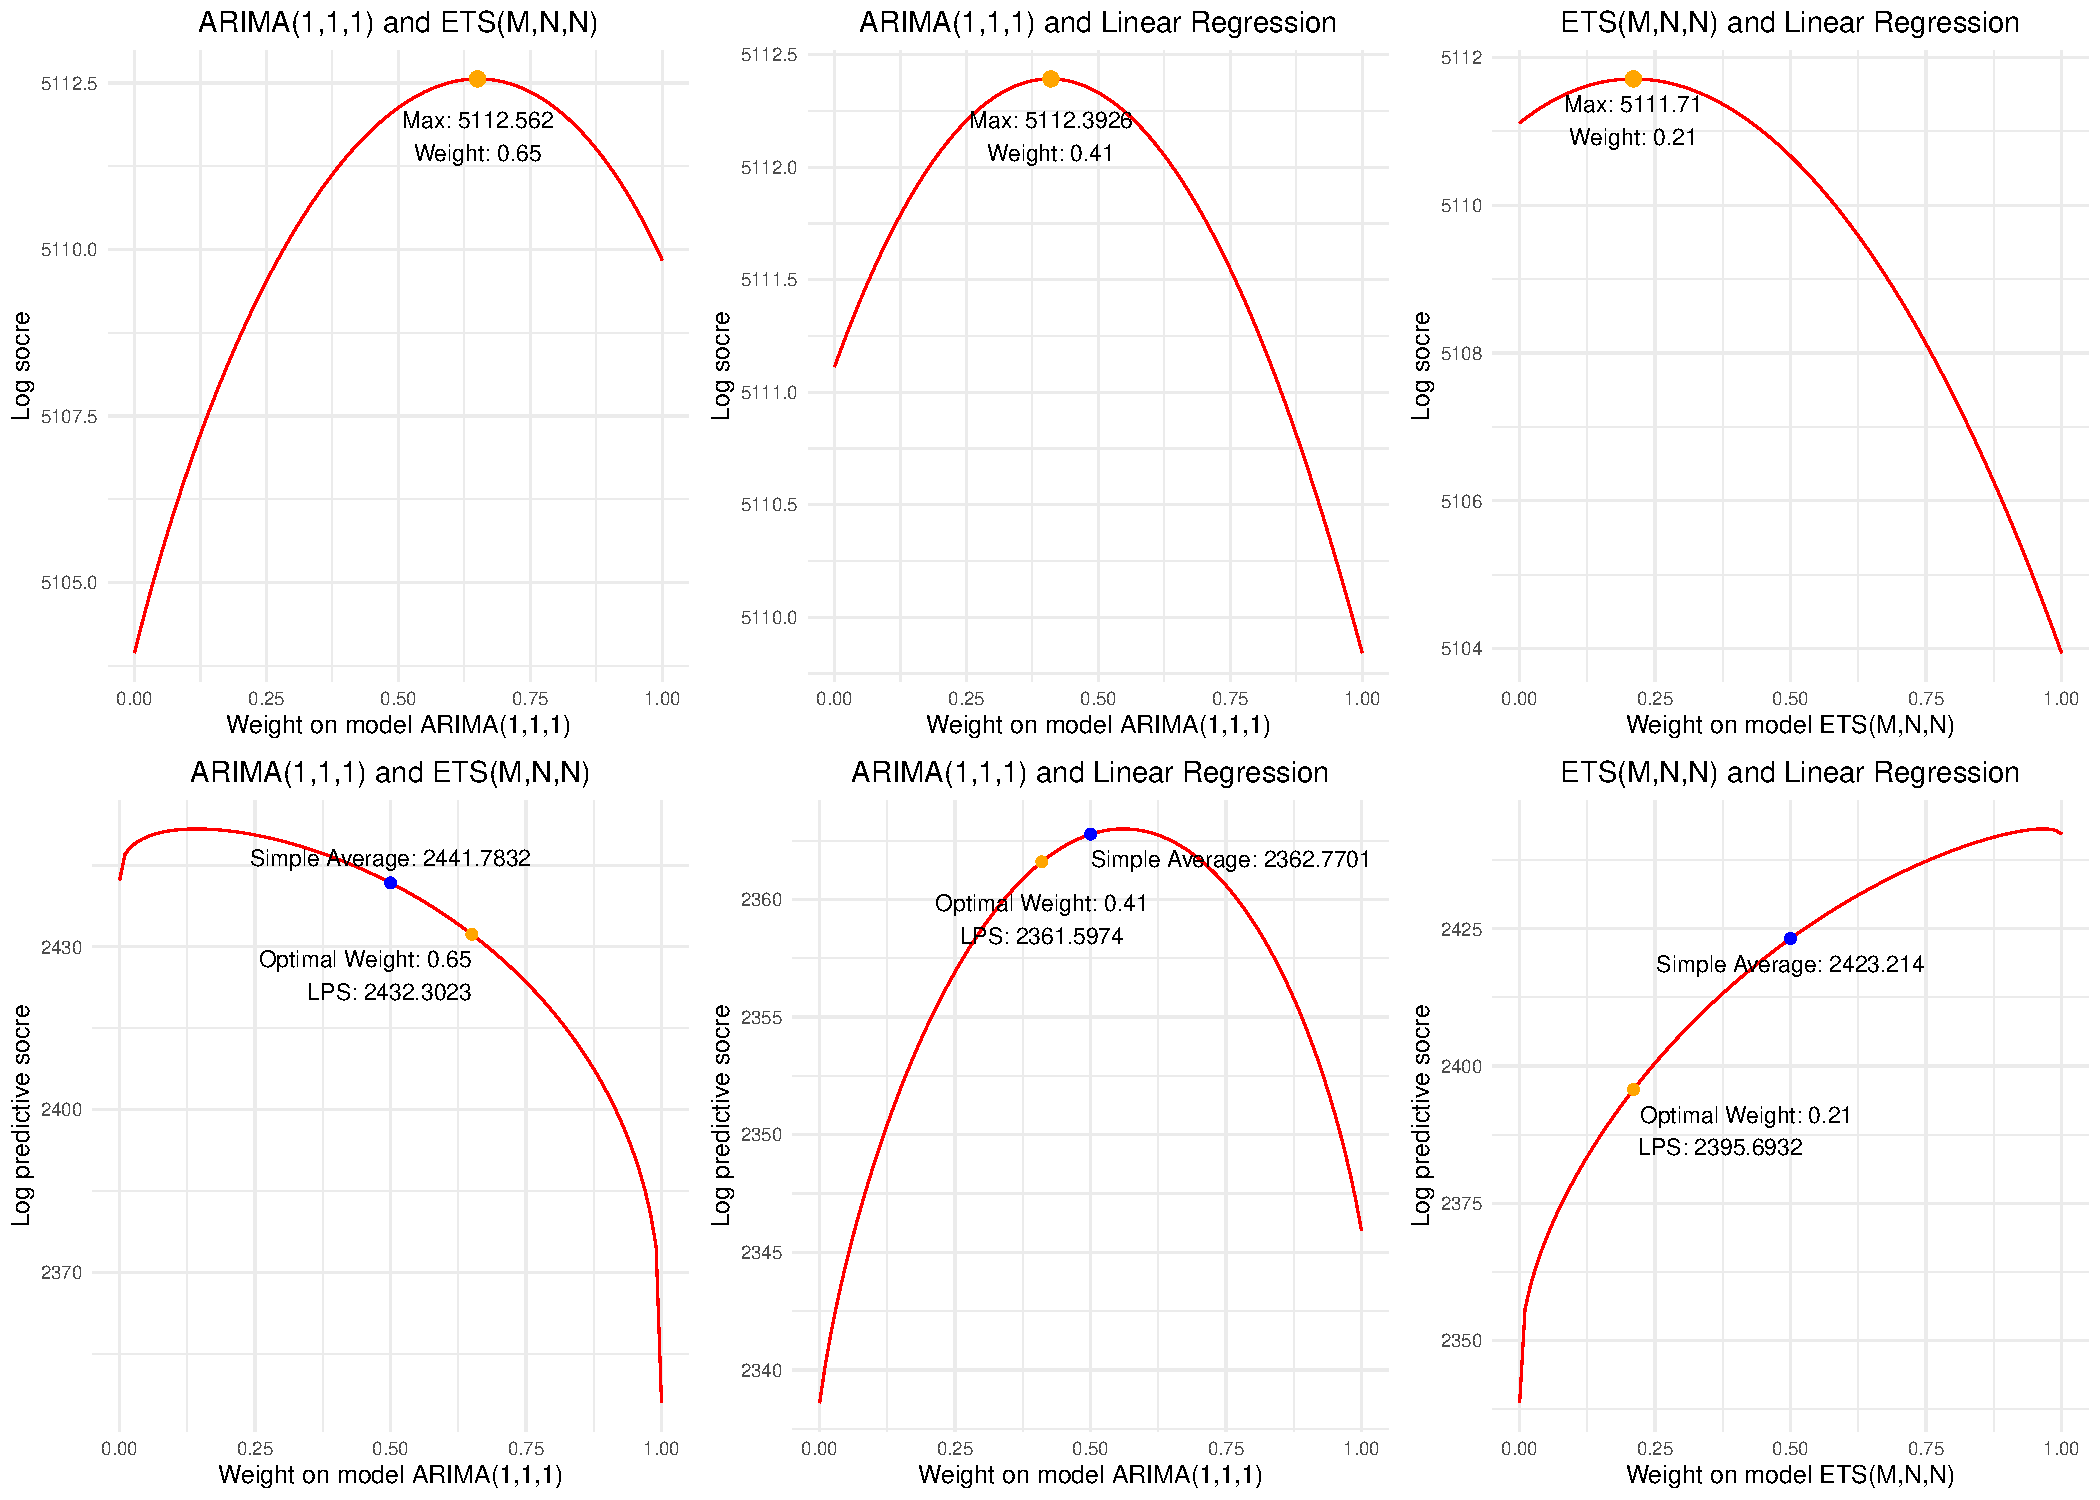
\includegraphics[scale=0.45]{figures/SP500_nonstationary.pdf}
\caption{Log predictive score of S\&P 500 index predictive densities in two-model pools over the in-sample (top) and out-of-sample (bottom) period. Constituent prediction models described in the title. The x-axis represents the weight assigned on the former model of the combination and the y-axis indicates the log predictive score. The orange dot represents the optimal combination, while the blue dot indicates the simple average.}
\label{fig:nonstat}
\end{figure}

Figure \ref{fig:nonstat} suggests that the forecast combination puzzle is evidenced in all three cases, where the simple average performs better out-of-sample than the optimal combination to different degrees. However, the difference in the log predictive score between two combination methods is varying for each case, and is very likely to be influenced by the in-sample fit of the constituent models. Relevant values are calculated and presented in Table \ref{tab:comparison1}. It is noticeable that when both models fit the data equally well, i.e., a small difference in the in-sample log score, the prediction accuracy of optimal and simple average approaches is very close. Meanwhile, the optimal forecast combination with a significant gap between the individual in-sample fit ends up performing worse than the mean of forecast densities.

\begin{table}[ht]
  \centering
    \begin{tabular}{l|ccc}
    \toprule
                                      &    Left     &   Middle    &    Right   \\
    \midrule
    In-sample log score difference    &   5.8989    &   1.2718    &   7.1707   \\
    Optimal versus average            &   9.9569    &   0.2268    &  19.9928   \\
    Presence of the puzzle            &   Yes       &   Yes       &   Yes      \\
    \bottomrule
    \end{tabular}
  \caption{``Left``, ``Middle`` and ``Right`` correspond to the position of each pair of combination in Figure \ref{fig:nonstat}. ``In-sample log score difference`` denotes the absolute difference of the log score over the training period between two models, which can be viewed as an informal accuracy measure of in-sample fit. ``Optimal versus average`` shows the absolute difference in log predictive score between the optimal combination and the simple average.}
  \label{tab:comparison1}
\end{table}

\begin{table}[ht]
  \centering
    \begin{tabular}{l|ccc}
    \toprule
                                      &        Left        &     Middle     &    Right       \\  
    \midrule
    First Model Log Likelihood        &     5113.694       &    5113.694    &   1725.137     \\
    Second Model Log Likelihood       &     1725.137       &    5116.014    &   5116.014     \\
    Log Likelihood Difference         &     3388.556       &     2.320      &   3390.876     \\
    Optimal Weight                    &       0.65         &      0.41      &     0.21       \\
    Puzzle                            &       Yes          &      Yes       &     Yes        \\
    \bottomrule
    \end{tabular}
  \caption{``Log Likelihood Difference`` represents the absolute difference of in-sample fit between two models, which is evaluated by the log likelihood. ``Optimal Weight`` is the estimated weight assigned to the first model in each combination. ``Puzzle`` indicates whether the simple average is close to or outperforms the optimal forecast combination.}
  \label{tab:nonfit}
\end{table}

One possible explanation could be that the ETS model fits the training set poorly compared to the other two models, while ARIMA and linear regression perform equally well. Based on the specification of ETS(M,N,N), we may argue that it fails to capture the trend component, shown in Figure \ref{fig:llg}, and is therefore a \texttt{Bad} model in the combination. On the other hand, the ARIMA and linear regression can be viewed as \texttt{Good} models.

\begin{figure}[ht]
\centering
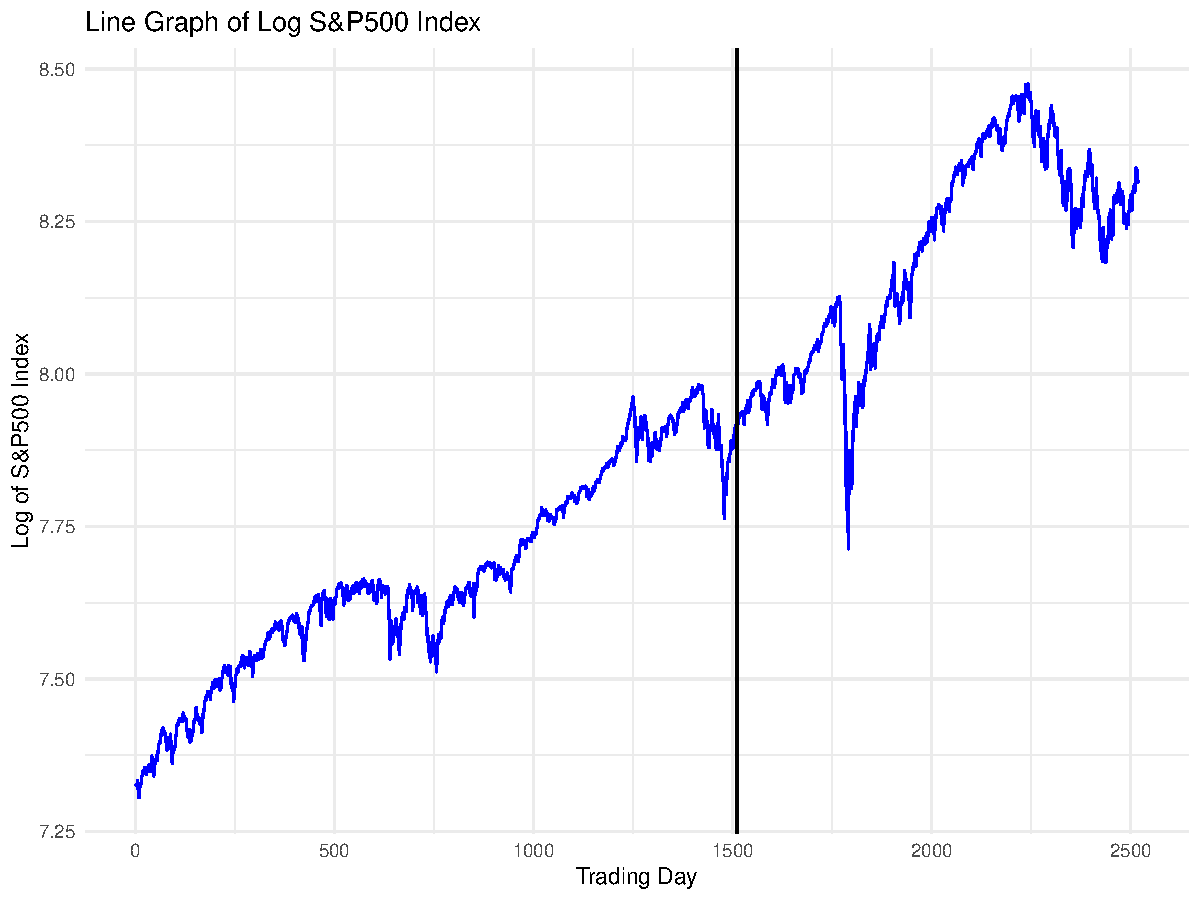
\includegraphics[scale=0.4]{figures/log_linegraph.pdf}
\caption{The black vertical line separates the traning set and the evaluation set. The training set is on the left and the evaluation set is on the right.}
\label{fig:llg}
\end{figure}

\hypertarget{stationary-time-series}{%
\subsection{Stationary time series}\label{stationary-time-series}}

Continuing with the same dataset, we now take a first difference of the log of S\&P 500 index, to construct log-returns, and then fit this covariance stationary series. A series is said to be covariance stationary when it has constant mean and variance, and its covariance depends on the time interval only.

Consider two candidate models: a Gaussian ARMA(1,1) model and a classical linear regression model with intercept only and ARMA(1,1) errors. To differentiate with the first linear regression model, it is named as Linear Regression 2 in the combination. Figure \ref{fig:stat} illustrates that two constituent models have a very similar in-sample log score, only 0.0011 difference, and the puzzle is evidenced given only 0.1282 accuracy difference between two forecast combination approaches.

\begin{figure}[ht]
\centering
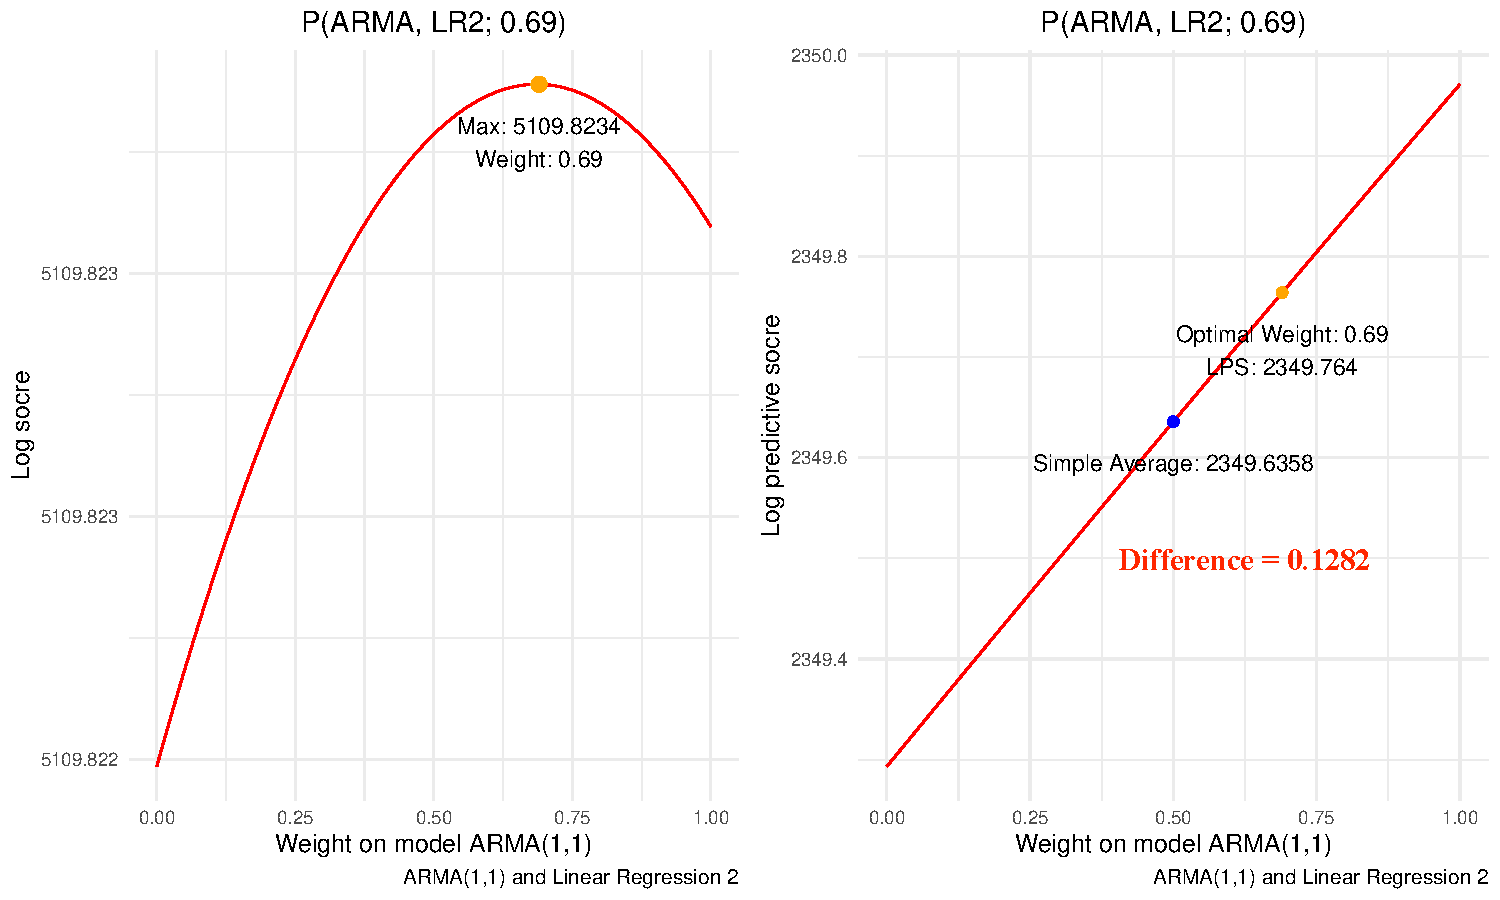
\includegraphics[scale=0.6]{figures/SP500_stationary.pdf}
\caption{Log predictive score of S\&P 500 index predictive densities in two-model pools over the in-sample (left) and the out-of-sample (right) period. The x-axis represents the weight assigned on the ARMA(1,1) model and the y-axis indicates the log predictive score. The meanings of colored dots remain the same as before.}
\label{fig:stat}
\end{figure}

\begin{table}[ht]
  \centering
    \begin{tabular}{l|ccc}
    \toprule
                                      &   ARMA(1,1) and Linear Regression 2   \\  
    \midrule
    First Model Log Likelihood        &               5109.8071               \\
    Second Model Log Likelihood       &               5109.8054               \\
    Log Likelihood Difference         &              0.001645751              \\
    Optimal Weight                    &                0.69                   \\
    Puzzle                            &                 Yes                   \\
    \bottomrule
    \end{tabular}
  \caption{``Log Likelihood Difference`` represents the absolute difference of in-sample fit between two models, which is evaluated by the log likelihood. ``Optimal Weight`` is the estimated weight assigned to the first model in each combination. ``Puzzle`` indicates whether the simple average is close to or outperforms the optimal forecast combination.}
  \label{tab:statfit}
\end{table}

This Section \ref{sp500} provides a little empirical evidence for our initial conjecture. When both models fit the data well, i.e., they are \texttt{Good} models, then the average density forecast performs almost the same as or slightly better than the optimal density forecast combination, indicating the presence of the forecast combination puzzle. If one model is \texttt{Bad} and the other is \texttt{Good}, then, at least, the puzzle can be evidenced.

\hypertarget{pure-time-series-with-seasonality}{%
\section{Pure time series with seasonality}\label{pure-time-series-with-seasonality}}

With the purpose of further examining our conjecture as to when the puzzle will be in evidence, we now use a quarterly dataset to explore the relationship between the forecast combination puzzle and in-sample model fit. More specifically, we investigate cases where both models are both well-specified (good) or poorly-specified (bad). To simplify the analysis, we produce point forecasts and evaluate point combinations with MSFE.

The data considered is the recorded quarterly total number of unemployed individuals (in thousands) from 1985 Q1 to 2023 Q1, retrieved from the Australia Bureau of Statistics \autocite{ABS}. It has a total of 153 (\(T\)) observations and is slit into two sets in proportion. Same as before, the first 60\% of the data (\(R = 91\)), as the in-sample period, is used to estimate all unknown parameters. The rest 40\% (\(P = 62\)) is the out-of-sample period for the forecast performance evaluation. Also, we use the natural logarithm of the total number of unemployment to reduce the level of variability in the series.

\hypertarget{well-specified-models}{%
\subsection{Well-specified models}\label{well-specified-models}}

To ensure compatibility with seasonal component, we propose the Seasonal ARIMA (SARIMA) model and the ETS model: ARIMA(2,0,2)(0,1,1){[}4{]} with drift and ETS(A,A,A). The SARIMA is simply an ARIMA model with extra seasonal component. The first parenthesis is same as before. The second parenthesis represents the seasonal AR, integrated, and MA components respectively, separately by the comma. The number in the box bracket indicates the number of observations per year, i.e., the seasonal frequency. An intercept is included in the model. In the ETS model, the seasonal part is reflected by \texttt{S} and the third position in the parenthesis. Due to the log transformation, we have additive error, additive trend, and additive seasonality.

The forecast combination puzzle is evidenced when both models are good in Figure \ref{fig:sd}. The optimal forecast point combination has a MSFE of 0.000177 and the simple averaging forecast has a MSFE of 0.000178. The difference between them is negligible. Looking at the in-sample combination plot, two models fit the training set equally well with a difference of 0.00000053. These results exemplify that two \texttt{Good} models in a two-model pool will close to having the forecast combination puzzle.

\begin{figure}[ht]
\centering
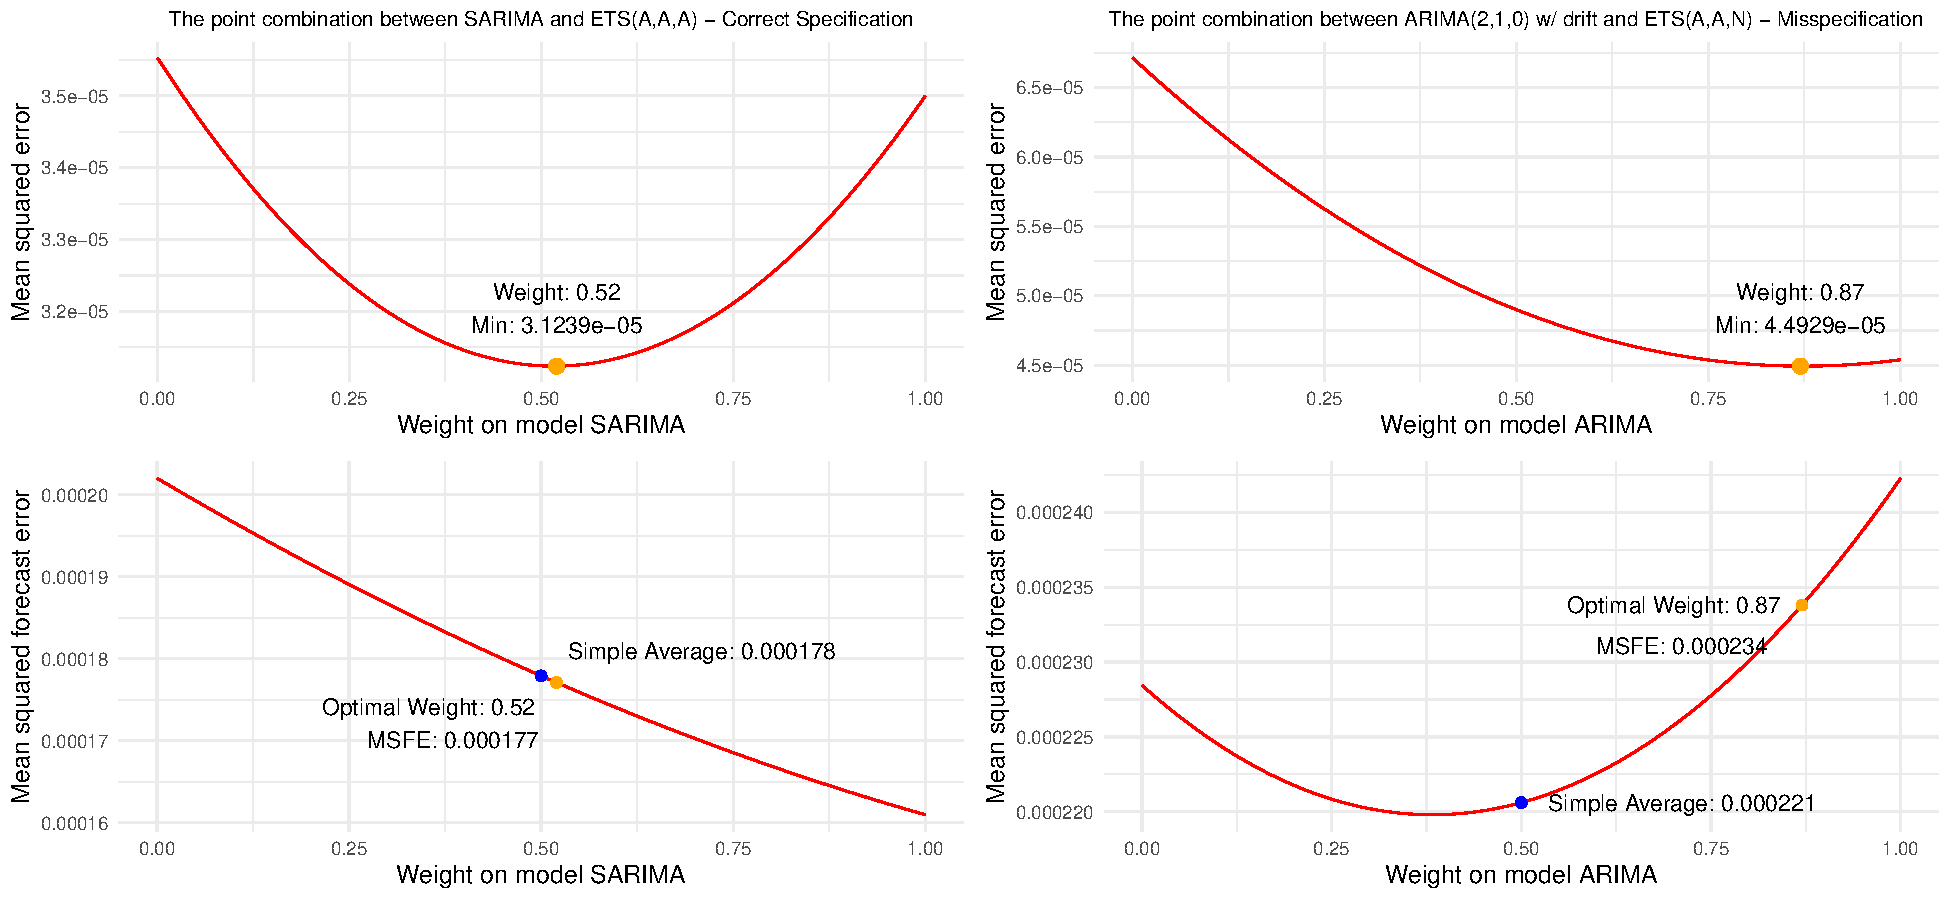
\includegraphics[scale=0.5]{figures/EMPL.pdf}
\caption{MSFE of predictive points in well-specified (left) and pooly-specified (right) two-model pools over the in-sample (top) and out-of-sample (bottom) period. The x-axis represents the weight assigned on the first model and the y-axis indicates the value of MSFE. The meanings of colored dots remain the same.}
\label{fig:sd}
\end{figure}

\hypertarget{poorly-specified-models}{%
\subsection{Poorly-specified models}\label{poorly-specified-models}}

One way of proposing a \texttt{Bad} model for a seasonal dataset is deliberately ignoring the seasonality in the model specification. Even so, we still try to fit the training set well with SARIMA and ETS models but only discarding their seasonal components: ARIMA(2,1,0) with an intercept and ETS(A,A,N).

The right column of Figure \ref{fig:sd} illustrates that both models have a similar in-sample performance with a deviation of 0.00002175. Furthermore, Figure \ref{fig:sd} does reveal the forecast combination puzzle, as the simple average performs more superior than the optimal forecast combination with a lower MSFE.

\begin{table}[ht]
  \centering
    \begin{tabular}{l|ccc}
    \toprule
                                      &   Well-specified   &   Poorly specified  \\  
    \midrule
    First Model Log Likelihood        &     321.4497       &        322.1642     \\
    Second Model Log Likelihood       &     260.9102       &        231.9507     \\
    Log Likelihood Difference         &     60.5395        &        90.2135      \\
    Optimal Weight                    &       0.52         &          0.87       \\
    Puzzle                            &       Yes          &          Yes        \\
    \bottomrule
    \end{tabular}
  \caption{``Log Likelihood Difference`` represents the absolute difference of in-sample fit between two models, which is evaluated by the log likelihood. ``Optimal Weight`` is the estimated weight assigned to the first model in each combination. ``Puzzle`` indicates whether the simple average is close to or outperforms the optimal forecast combination.}
  \label{tab:season}
\end{table}

In this case, we may claim that, regardless whether the constituent models capture all the features of the data, as long as they have similar in-sample fit, the forecast combination puzzle will be evidenced. As a result, even if we have two \texttt{Bad} models, if they have similar in-sample performance, we should expect to find the puzzle.

\hypertarget{simulation-results}{%
\chapter{Simulation Results}\label{simulation-results}}

\hypertarget{pure-cross-sectional-setting}{%
\section{Pure cross-sectional setting}\label{pure-cross-sectional-setting}}

Given that the forecast combination can greatly improve the forecast accuracy, this idea of model combination can also be applied to the cross-sectional setting. A simulated cross-sectional dataset is designed to study how elements in the linear regression model affect the presence of the puzzle, as well as the performance of density combinations. Instead of using real-life data, implementing simulation is easy to control and to make any changes efficiently. At the same time, it is an effective way of validating our conjectures through exploring the forecast combination puzzle from different aspects. In line with previous notations but in the cross-sectional setting, the subscript \texttt{t} will change to \texttt{i} to represent each individual observation.

\hypertarget{experimental-design}{%
\subsection{Experimental design}\label{experimental-design}}

The true data-generating process (DGP) is assumed to be a linear regression model with only two exogenous and correlated regressors, which satisfies all classical assumptions:

\begin{equation}
\label{eqn:DGP}
y_i = \beta_0 + \beta_1 x_{1i} + \beta_2 x_{2i} + e_i, \ \ e_i \stackrel{i.i.d}{\sim} N(\mu_e,\sigma^2_e) \\
\end{equation}

where \(i\) represents each observation.

The initial set-up has 1000 (N) artificial cross-sectional observations generated from \ref{eqn:DGP} with \(E[x_{1i}] = E[x_{2i}] = 0\), \(Var(x_{1i}) = Var(x_{2i}) = 1\), \(Cov(x_{1i}, x_{2i}) = 0.7\), \(\pmb{\beta} = (\beta_0, \beta_1, \beta_2)' = (1,2,2)'\), \(\mu_e = 0\) and \(\sigma^2_e=4\).

Following the methodology in Section \ref{method}, the data will be divided into an in-sample period (roughly 60\%) for estimation and an out-of-sample period for accuracy evaluation. We propose two pooly-specified models to generate density forecasts with each contains only one of the regressors. Assume Model 1 \(M_1\) purely includes \(x_{1i}\) as the regressor and Model 2 \(M_2\) only has \(x_{2i}\) as the regressor. The density forecast combinations will follow the construction of \texttt{two-model} pools and be evaluated using the log score.

\begin{figure}[ht]
\centering
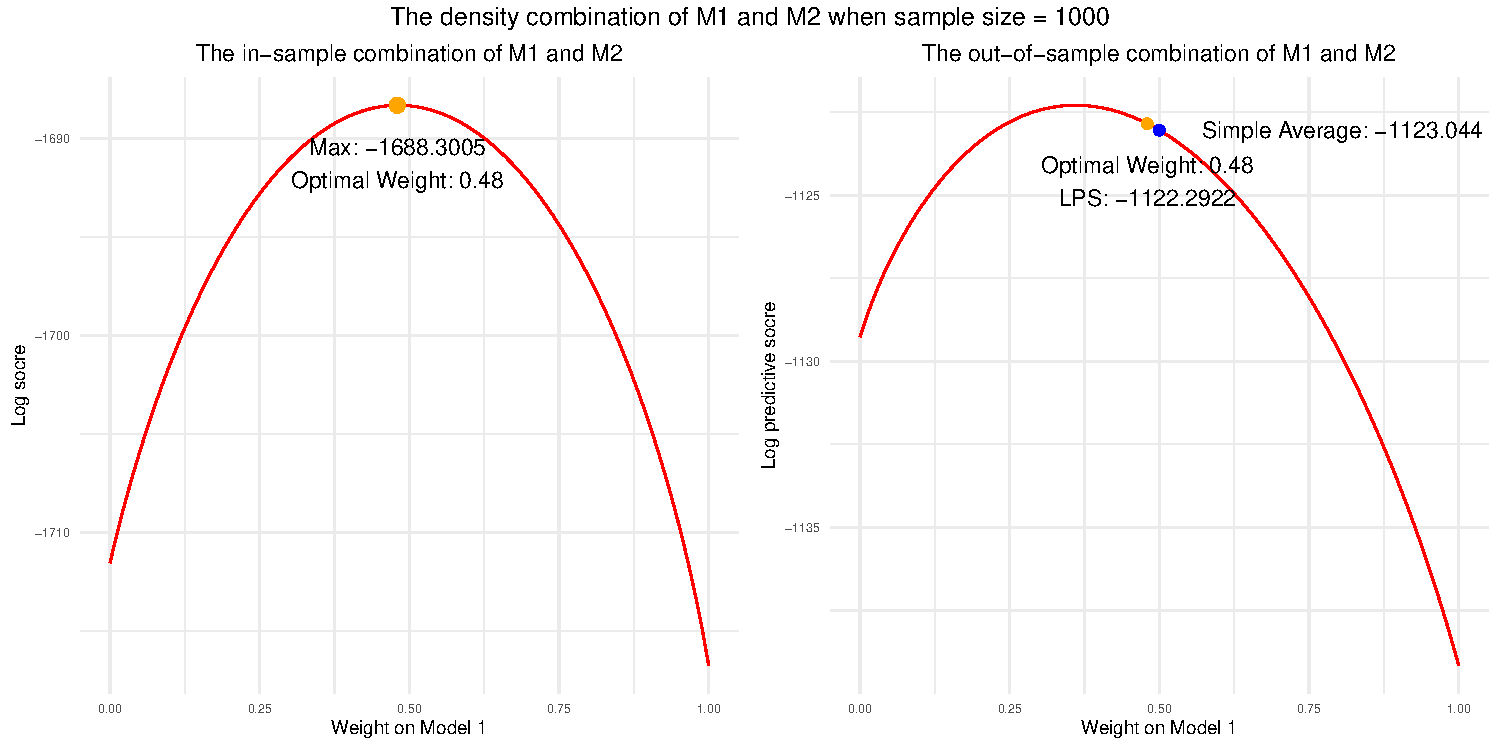
\includegraphics[scale=0.6]{figures/ss_1000.pdf}
\caption{Two curves refer to the in-sample (left) and out-of-sample (right) performance of density combinations with artificial cross-sectional data based on the initial set-up. The x-axis represents the weight assigned on Model 1 and the y-axis indicates the log score for each density combination. The orange dot represents the optimal forecast combination, while the blue dot indicates the forecast performance of the simple average combination.}
\label{fig:ss1000}
\end{figure}

Figure \ref{fig:ss1000} clearly shows that when the sample size is large and two models have similar in-sample performance, the forecast accuracy will be indistinguishable between the simple average of predicted densities and the optimal density forecast combination, which is a strong evidence of the forecast combination puzzle. We can then change the true value of different elements, and determine the conditions under which the puzzle is likely to be evidenced. More rigorously, we will evaluate the in-sample performance with the \(R^2\) of constituent models, and then analyse its relationship with the optimal combination weight and the presence of the puzzle.

\begin{itemize}
\tightlist
\item
  \bf{Sample Size}
\end{itemize}

\begin{figure}
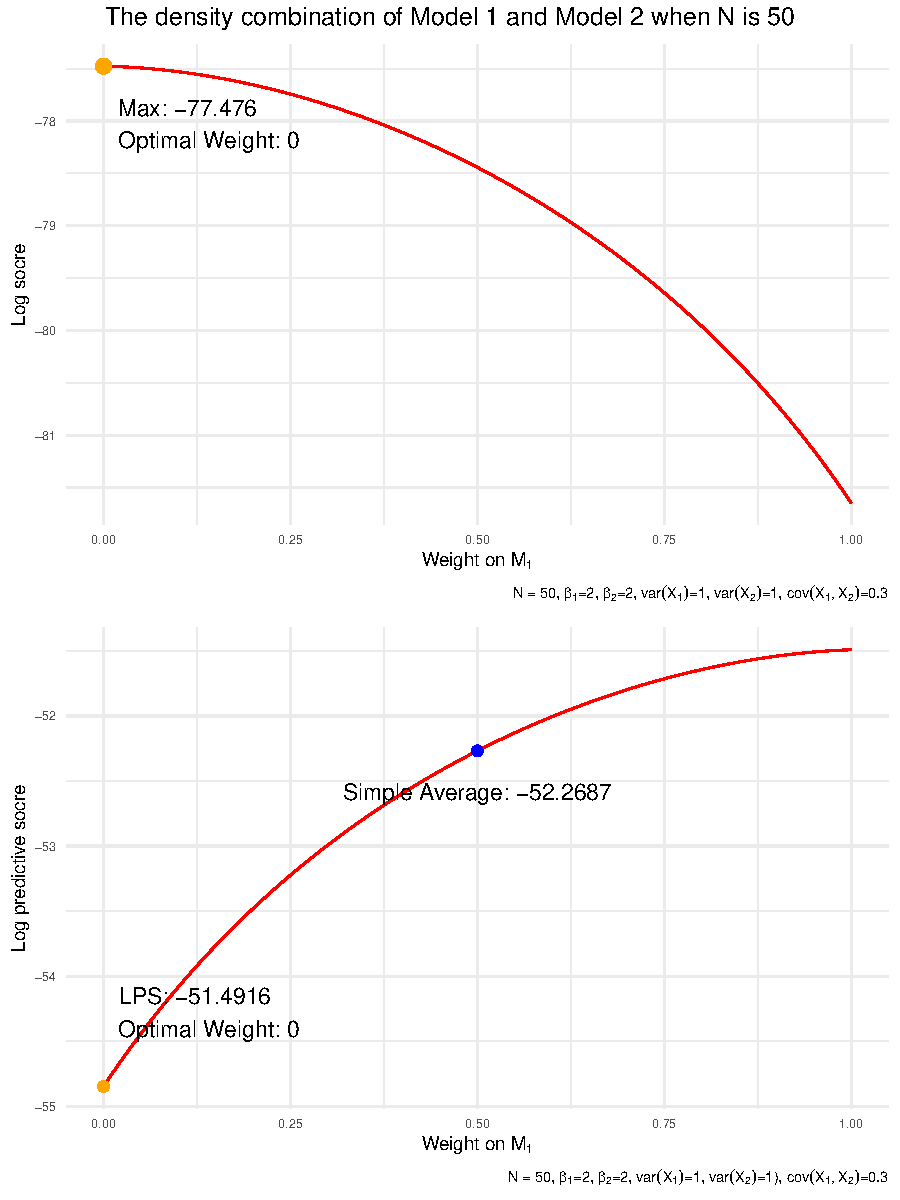
\includegraphics[width=0.47\textwidth]{figures/ss_50.pdf}
\hspace{\fill}
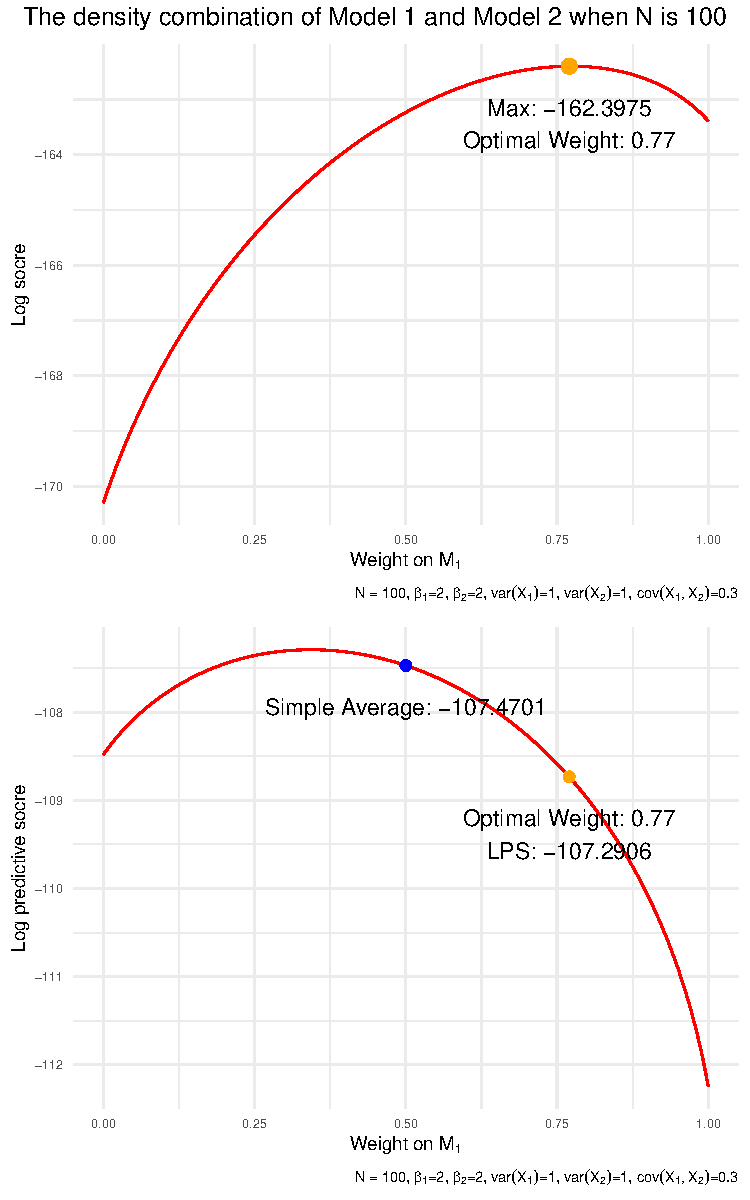
\includegraphics[width=0.47\textwidth]{figures/ss_100.pdf}
\caption{Two columns refer to the in-sample combination performance (top) and the out-of-sample combination accuracy (bottom) when $N=100$ and $N=1000$ while keeping all others the same as in the initial set-up. The meanings of colored dots are the same as those in Figure \ref{fig:ss1000}.}
\label{fig:samplesize}
\end{figure}

From Figure \ref{fig:samplesize}, it is noticeable that the set of optimal weight varies a lot when we have different sample sizes. Model 1 is given an extremely low weight when \(N=50\) whereas it is highly preferred when \(N=100\). The optimal weight is 0.48 when the sample size becomes 1000, shown in Figure \ref{fig:ss1000}. Based on the log score curve of in-sample combinations, the optimal weight is highly correlated with the individual model performance. The number of observations can be viewed as one factor that can affect the model fit. Figure \ref{fig:samplesize} also shows that the average density forecast performs much better than the optimal density combination in both cases, i.e., the forecast combination puzzle is found.

\begin{table}[ht]
  \centering
    \begin{tabular}{l|ccc}
    \toprule
    Sample Size      &   $N=50$    &    $N=100$   &  $N=1000$  \\
    \midrule
    $R^2$ of $M_1$   &   0.4928    &    0.4953    &   0.3612   \\
    $R^2$ of $M_2$   &   0.5620    &    0.3320    &   0.3722   \\
    Difference       &   0.0692    &    0.1633    &   0.0110   \\
    Optimal Weight   &    0.07     &     0.98     &    0.48    \\
    Puzzle           &    Yes      &     Yes      &    Yes     \\
    \bottomrule
    \end{tabular}
  \caption{``Difference`` represents the absolute difference of in-sample fit between two models. ``Optimal Weight`` is the estimated weight assigned to $M_1$. ``Puzzle`` indicates whether the simple average is close to or outperforms the optimal forecast combination.}
  \label{tab:size}
\end{table}

Table \ref{tab:size} illustrates that when two models have a relatively big difference in the in-sample fit \(R^2\) (in the second and third columns), we are then more likely to have an extreme optimal weight \(\omega\). However, when two models have similar \(R^2\) in the fourth column, the optimal weight \(\omega\) is close to 0.5. These empirical results first support the conjecture that when models have indifferent in-sample fit, the puzzle is likely evidenced. Additionally, they illustrate that the puzzle can be in evidence when one model performs outstandingly.

\begin{itemize}
\tightlist
\item
  \bf{Magnitude and Sign of $\pmb{\beta}$}
\end{itemize}

Next, we explore the effect changes in magnitudes or signs of \(\beta_1\) and \(\beta_2\) given two different sample sizes. From here on, combination plots will be collected and displayed in Appendix \ref{plot}. According to Figure \ref{fig:magnitude}, the puzzle is highly sensitive to the absolute difference between two parameters. If the absolute difference is large enough, generally more than half of the smaller coefficient, it is hard to find the puzzle and the optimal combination always wins with a higher log predictive score. In the linear regression analysis, the magnitude of coefficient represents the impact size of corresponding regressor on the dependent variable. A large value of coefficient means that a change in the regressor will affect the dependent variable more in magnitude. Knowing this, it is reasonable to observe that the Model 1 has a decreasing weight in the optimal combination from left to right in Figure \ref{fig:magnitude}. The effect of \(x_{2i}\) on \(y_i\), \(\beta_2\), is relatively larger than the effect of \(x_{1i}\) on \(y_i\), \(\beta_1\), so the Model 2 with \(x_{2i}\) should be weighted higher in the combination.

\begin{table}[ht]
  \centering
    \begin{tabular}{l|cccc}
    \toprule
    Different Magnitudes    &  $\beta_1=2,\ \beta_2=4$   &  $\beta_1=2,\ \beta_2=6$ &  $\beta_1=2,\ \beta_2=4$  &  $\beta_1=2,\ \beta_2=6$  \\
    \midrule
    $R^2$ of $M_1$  &    0.6516    &   0.7057   &    0.4567     &   0.4948   \\
    $R^2$ of $M_2$  &    0.6043    &   0.7574   &    0.6082     &   0.7478   \\
    Difference      &    0.0472    &   0.0517   &    0.1516     &   0.2530   \\
    Optimal Weight  &     0.59     &    0.32    &     0.18      &    0.04    \\
    Puzzle          &     Yes      &     No     &      No       &     No     \\
    Sample Size     &     100      &    100     &     1000      &    1000    \\
    \bottomrule
    \end{tabular}
  \caption{``Difference`` represents the absolute difference of in-sample fit between two models. ``Optimal Weight`` is the estimated weight assigned to $M_1$. ``Puzzle`` indicates whether the simple average is close to or outperforms the optimal forecast combination.}
  \label{tab:bmag}
\end{table}

With reference to the previous results, when the absolute difference is small, the optimal weight \(\omega_{opt}\) is expected to be around 0.5 and we are expected to find the puzzle. The second column of Table \ref{tab:bmag} provides another empirical evidence where the absolute difference is around 0.0472. The other three cases, however, illustrate the results when the absolute difference of \(R^2\) is big enough. Different from the cases in the second and third columns of Table \ref{tab:size}, the puzzle is not obvious when one model is more favored, and we have the optimal forecast combination outperforms the simple average forecast. Recall our initial conjecture about the combination of a \texttt{Good} model and a \texttt{Bad} model, simulations have shown some corroborating evidence that the puzzle is ambiguous.

Table \ref{tab:bsig} further justifies our conjecture of the relationship between the in-sample performance and the presence of the puzzle. Especially when the sample size is 100, there is a huge difference between the in-sample fit of two models and \(M_2\) is given all the weight in the optimal combination. This clearly implies that the puzzle is not discovered randomly but related to the model in-sample performance. It is also noticeable that conditioning on the same magnitude, the sample size has a large impact on the model fit. When the sample size is small, the absolute difference of in-sample performance becomes larger, leading to an extreme optimal weight and the presence of the puzzle is uncertain as well.

\begin{table}[ht]
  \centering
    \begin{tabular}{l|cccc}
    \toprule
    Different Signs &  $\beta_1=2,\ \beta_2=-2$  &  $\beta_1=4,\ \beta_2=-4$  &  $\beta_1=2,\ \beta_2=-2$  &  $\beta_1=4,\ \beta_2=-4$\\
    \midrule
    $R^2$ of $M_1$  &    0.0002    &   0.00002  &    0.0131     &   0.0423   \\
    $R^2$ of $M_2$  &    0.1130    &   0.1934   &    0.0321     &   0.0856   \\
    Difference      &    0.1128    &   0.1934   &    0.0191     &   0.0433   \\
    Optimal Weight  &      0       &     0      &     0.38      &    0.38    \\
    Puzzle          &      No      &     No     &      Yes      &    Yes     \\
    Sample Size     &     100      &    100     &     1000      &    1000    \\
    \bottomrule
    \end{tabular}
  \caption{``Difference`` represents the absolute difference of in-sample fit between two models. ``Optimal Weight`` is the estimated weight assigned to $M_1$. ``Puzzle`` indicates whether the simple average is close to or outperforms the optimal forecast combination.}
  \label{tab:bsig}
\end{table}

\begin{itemize}
\tightlist
\item
  \bf{Variance of regressors}
\end{itemize}

We keep the variance of \(x_{2i}\) the same value and only increase the variance of \(x_{1i}\). Then \(x_{1i}\) should have a larger variance than \(x_{2i}\), thus the variation of \(y_i\) can be explained more by Model 1 than Model 2. This can be verified by Table \ref{tab:regvar} where \(R^2\) of \(M_1\) is always higher than that of \(M_2\). Consequently, the in-sample performance difference between the two models is big enough to presume that all four combinations include a \texttt{good} Model 1 and a \texttt{bad} Model 2. As expected in the conjecture, Model 1 should have a higher weight, far away from 0.5, in the optimal combination. Furthermore, the forecast combination puzzle is evidenced in three of them while it is not found in the last situation, indicating that the presence of the puzzle is unclear when there is a big gap in the in-sample fit.

\begin{table}[ht]
  \centering
    \begin{tabular}{l|cccc}
    \toprule
    Change in Variance of $x_{1i}$    &  $Var(x_{1i}) = 2$   &  $Var(x_{1i}) = 4$  &  $Var(x_{1i}) = 2$  &  $Var(x_{1i}) = 4$  \\
    \midrule
    $R^2$ of $M_1$  &    0.5389    &   0.6056   &    0.3981     &   0.4947   \\
    $R^2$ of $M_2$  &    0.2899    &   0.2464   &    0.3225     &   0.2536   \\
    Difference      &    0.2490    &   0.3592   &    0.0756     &   0.2411   \\
    Optimal Weight  &     0.92     &    0.94    &     0.66      &    0.85    \\
    Puzzle          &      Yes     &    Yes     &      Yes      &     No     \\
    Sample Size     &     100      &    100     &     1000      &    1000    \\
    \bottomrule
    \end{tabular}
  \caption{``Difference`` represents the absolute difference of in-sample fit between two models. ``Optimal Weight`` is the estimated weight assigned to $M_1$. ``Puzzle`` indicates whether the simple average is close to or outperforms the optimal forecast combination.}
  \label{tab:regvar}
\end{table}

One additional hypothesis is that when the absolute difference of \(R^2\) between two models is less than 0.05, they should be treated as having similar in-sample performance. \textbf{Formally, the null hypothesis is that the absolute difference of the in-sample fit \(R^2\) is less than 0.05.}

These results provide a general idea of the relationship between the in-sample fit of constituent models and the presence of the forecast combination puzzle. Based on the new information, the conjecture for two-model pools should be updated, as illustrated in Table \ref{tab:2}.

\begin{table}[ht]
\centering
\begin{tabular}{lcc}
Absolute difference of in-sample fit    &     Small      &    Large    \\
Presence of the puzzle                  &     $\surd$    &    $?$      \\
\end{tabular}
\caption{``Small`` means that both models fit the in-sample data equally well (or equally bad), whereas ``Large`` implies that one of the models performs poorly in fitting the training set. The ``$\surd$`` implies the presense of the forecast combination puzzle, while ``$?$`` means that the presense of the puzzle is ambiguous.}
\label{tab:2}
\end{table}

The choice of model is arbitrary and only the two-model pool is considered. It is also not prudent to determine \texttt{small} and \texttt{Large} difference based on subjective opinions. Potential improvements include\ldots{}

\hypertarget{discussion}{%
\chapter{Discussion}\label{discussion}}

\hypertarget{conclusion}{%
\chapter{Conclusion}\label{conclusion}}

Working in the two-model pools provides an opportunity of exploring a variety of situations in a short period of time. The next challenging step should naturally be to investigate the multiple forecasts combination, and we leave it to future research.

\appendix

\hypertarget{appendix}{%
\chapter{Appendix}\label{appendix}}

All codes are performed in R Statistical Software (version 4.2.1 (2022-06-23)). The packages used are \texttt{tidyverse} \autocite{tidy19}, \texttt{dplyr} \autocite{dplyr23}, \texttt{fpp3} \autocite{fpp23}, \texttt{gridExtra} \autocite{gridExtra}, and \texttt{mvtnorm} \autocite{GBMMLSH21}.

\hypertarget{model-specification}{%
\section{Model Specification}\label{model-specification}}

The error term, \(\epsilon_t\), in each model is assumed to be independent and normally distributed with a zero mean and a constant variance. Each model is independent. Even if using the same notation for unknown parameters across models, the estimators are different.

Exact formulas and explanations of these models can be found in \textcite{fpp3}. The formula of the conditional variance for the ETS(M,N,N) model is discussed in Chapter 6.3 of \textcite{HKOS08}.

\hypertarget{nonstationary-sp-500-index}{%
\subsection{Nonstationary S\&P 500 Index}\label{nonstationary-sp-500-index}}

\begin{enumerate}
\def\labelenumi{\arabic{enumi}.}
\item
  ARIMA(1,1,1) model with an intercept of the natural logarithm of S\&P 500 index.
  \begin{equation*}
  log(y_t) = c + log(y_{t-1}) + \phi_1\big[log(y_{t-1})-log(y_{t-2})\big] + \epsilon_t + \theta_1\epsilon_{t-1}
  \end{equation*}
\item
  ETS(M,N,N) model of the natural logarithm of S\&P 500 index.
  \begin{align*}
  log(y_t) &= \ell_{t-1} (1+\epsilon_t) \\
  \ell_t &= \ell_{t-1} (1+\alpha \epsilon_t) \\
  \end{align*}
\item
  A classical linear regression model of the natural logarithm of the S\&P 500 index and ARIMA(1,0,0) errors.
  \begin{align*}
  log(y_t) &= \beta_0 + \beta_1 t + u_t \\
  u_t &= \phi_1 u_{t-1} + \epsilon_t
  \end{align*}
\end{enumerate}

\hypertarget{stationary-sp-500-index}{%
\subsection{Stationary S\&P 500 Index}\label{stationary-sp-500-index}}

\begin{enumerate}
\def\labelenumi{\arabic{enumi}.}
\item
  ARMA(1,1) model with an intercept of the natural logarithm of S\&P 500 returns.
  \begin{equation*}
  log(y_t) - log(y_{t-1}) = c + \phi_1\big[log(y_{t-1})-log(y_{t-2})\big] + \epsilon_t + \theta_1\epsilon_{t-1}
  \end{equation*}
\item
  A classical linear regression model of the natural logarithm of the S\&P 500 returns and ARMA(1,1) errors.
  \begin{align*}
  log(y_t) &= \beta_0 + u_t \\
  u_t &= \phi_1 u_{t-1} + \epsilon_t + \theta_1\epsilon_{t-1}
  \end{align*}
\end{enumerate}

\hypertarget{well-specified-models-for-seasonal-unemployment-dataset}{%
\subsection{Well-specified models for seasonal unemployment dataset}\label{well-specified-models-for-seasonal-unemployment-dataset}}

\begin{enumerate}
\def\labelenumi{\arabic{enumi}.}
\item
  ARIMA(2,0,2)(0,1,1){[}4{]} model with an intercept of the natural logarithm of unemployed individuals.
  \begin{align*}
  log(y_t) &= c + log(y_{t-4}) + \phi_1\big[log(y_{t-1})-log(y_{t-5})\big] + \phi_2\big[log(y_{t-2})-log(y_{t-6})\big] \\
        &+ \epsilon_t + \theta_1\epsilon_{t-1} + \theta_2\epsilon_{t-2} + \Theta_1\epsilon_{t-4} + \theta_1\Theta_1\epsilon_{t-5} + \theta_2\Theta_1\epsilon_{t-6} \\
  \end{align*}
\item
  ETS(A,A,A) model of the natural logarithm of unemployed individuals.
  \begin{align*}
  log(y_t) &= \ell_{t-1} + b_{t-1} + s_{t-m} + \epsilon_t \\
  \ell_t &= \ell_{t-1} + b_{t-1} + \alpha \epsilon_t \\
  b_t &= b_{t-1} + \beta \epsilon_t \\
  s_{t} &= s_{t-m} + \gamma \epsilon_t
  \end{align*}
\end{enumerate}

\hypertarget{poorly-specified-models-for-seasonal-unemployment-dataset}{%
\subsection{Poorly-specified models for seasonal unemployment dataset}\label{poorly-specified-models-for-seasonal-unemployment-dataset}}

\begin{enumerate}
\def\labelenumi{\arabic{enumi}.}
\item
  ARIMA(2,1,0) model with an intercept of the natural logarithm of unemployed individuals.
  \begin{equation*}
  log(y_t) = c + log(y_{t-1}) + \phi_1\big[log(y_{t-1})-log(y_{t-2})\big] + \phi_2\big[log(y_{t-2})-log(y_{t-3})\big] + \epsilon_t
  \end{equation*}
\item
  ETS(A,A,N) model of the natural logarithm of unemployed individuals.
  \begin{align*}
  log(y_t) &= \ell_{t-1} + b_{t-1} + \epsilon_t \\
  \ell_t &= \ell_{t-1} + b_{t-1} + \alpha \epsilon_t \\
  b_t &= b_{t-1} + \beta \epsilon_t
  \end{align*}
\end{enumerate}

\hypertarget{plot}{%
\section{In-sample and out-of-sample combination plot}\label{plot}}

\begin{figure}[ht]
\centering
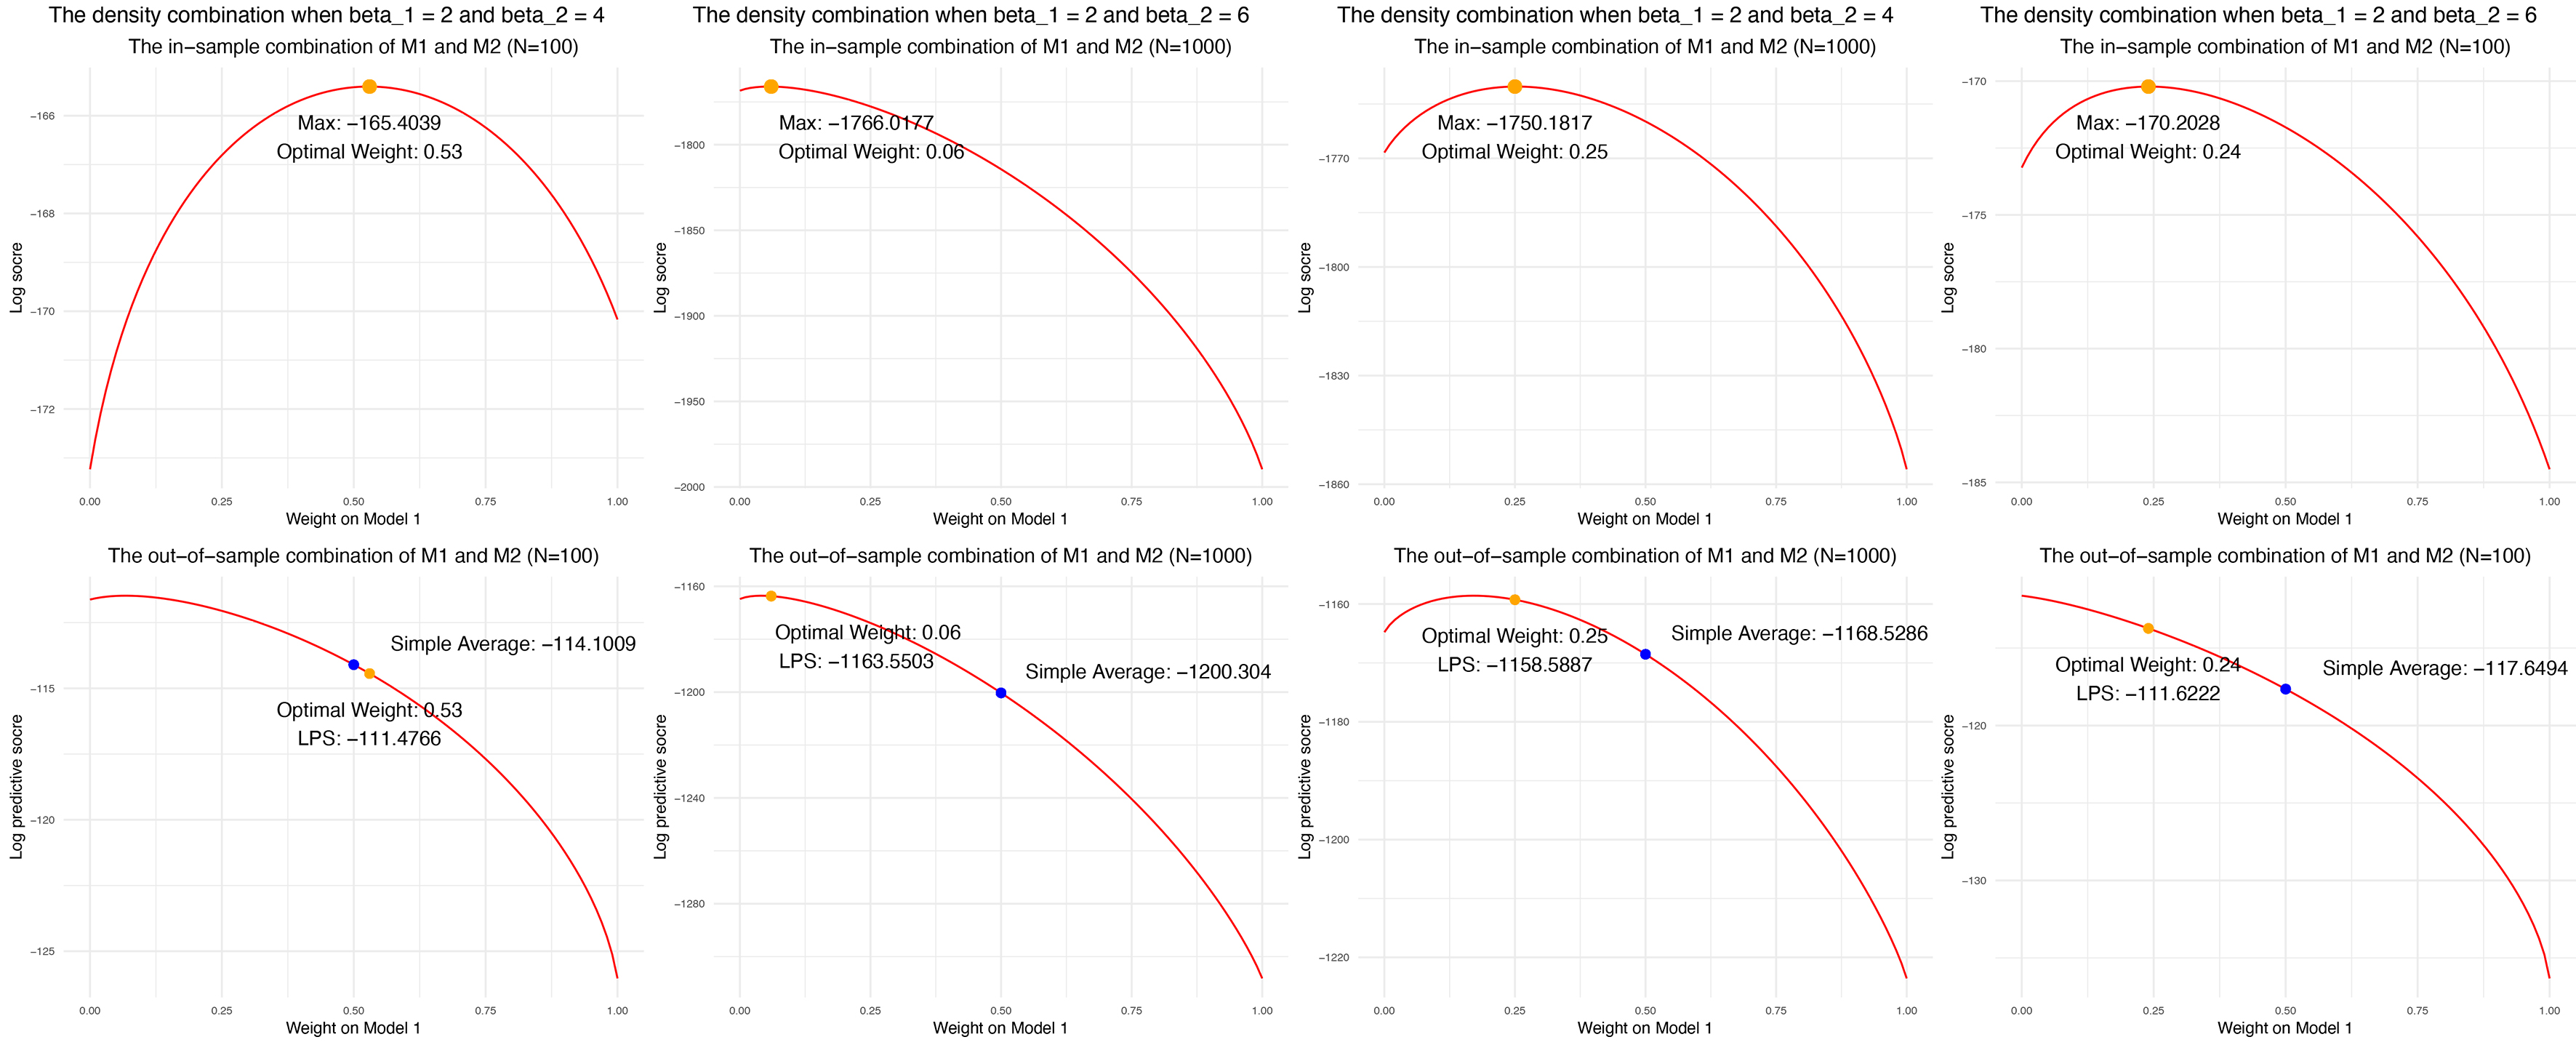
\includegraphics[scale=0.18, angle=90]{figures/betamag11.jpg}
\caption{$\beta_1$ and $\beta_2$ have the same sign but different magnitudes. The first and third columns $\beta_1=2$ and $\beta_2=4$, and the second and fourth columns $\beta_1=2$ and $\beta_2=6$. The sample size is indicated in the subtitle. Other variables remain unchanged as in the initial set-up.}
\label{fig:magnitude}
\end{figure}

\begin{figure}[ht]
\centering
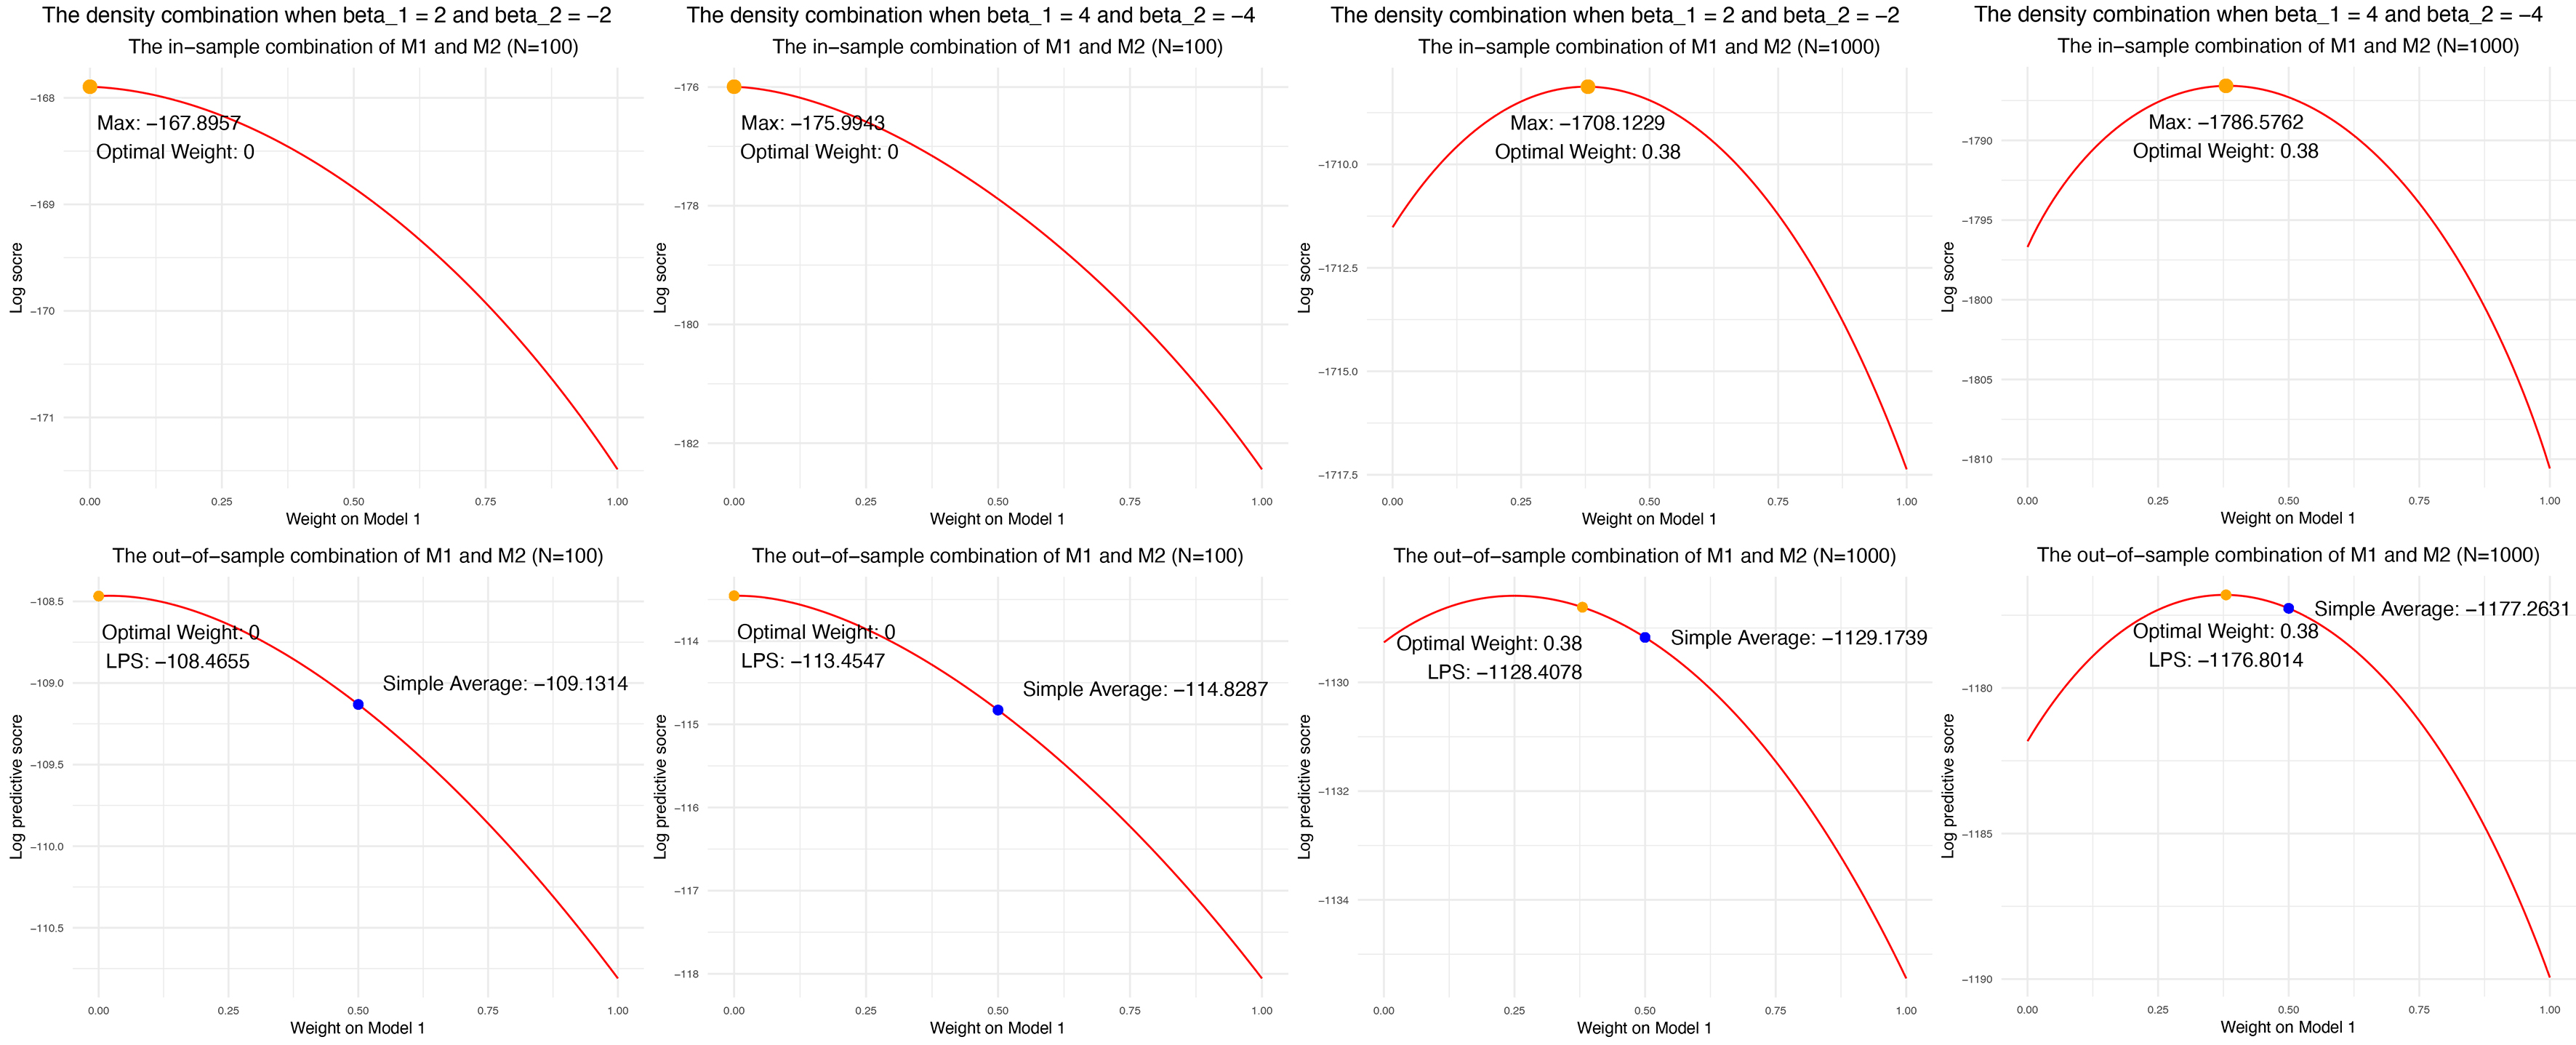
\includegraphics[scale=0.18, angle=90]{figures/betasign11.jpg}
\caption{$\beta_1$ and $\beta_2$ have the same magnitude but different signs, i.e. $\beta_1=-\beta_2$. The first and third columns $\beta_1=2$ and $\beta_2=-2$, and the second and fourth columns $\beta_1=4$ and $\beta_2=-4$. The sample size is indicated in the subtitle. Other variables remain unchanged as in the initial set-up.}
\label{fig:sign}
\end{figure}

\begin{figure}[ht]
\centering
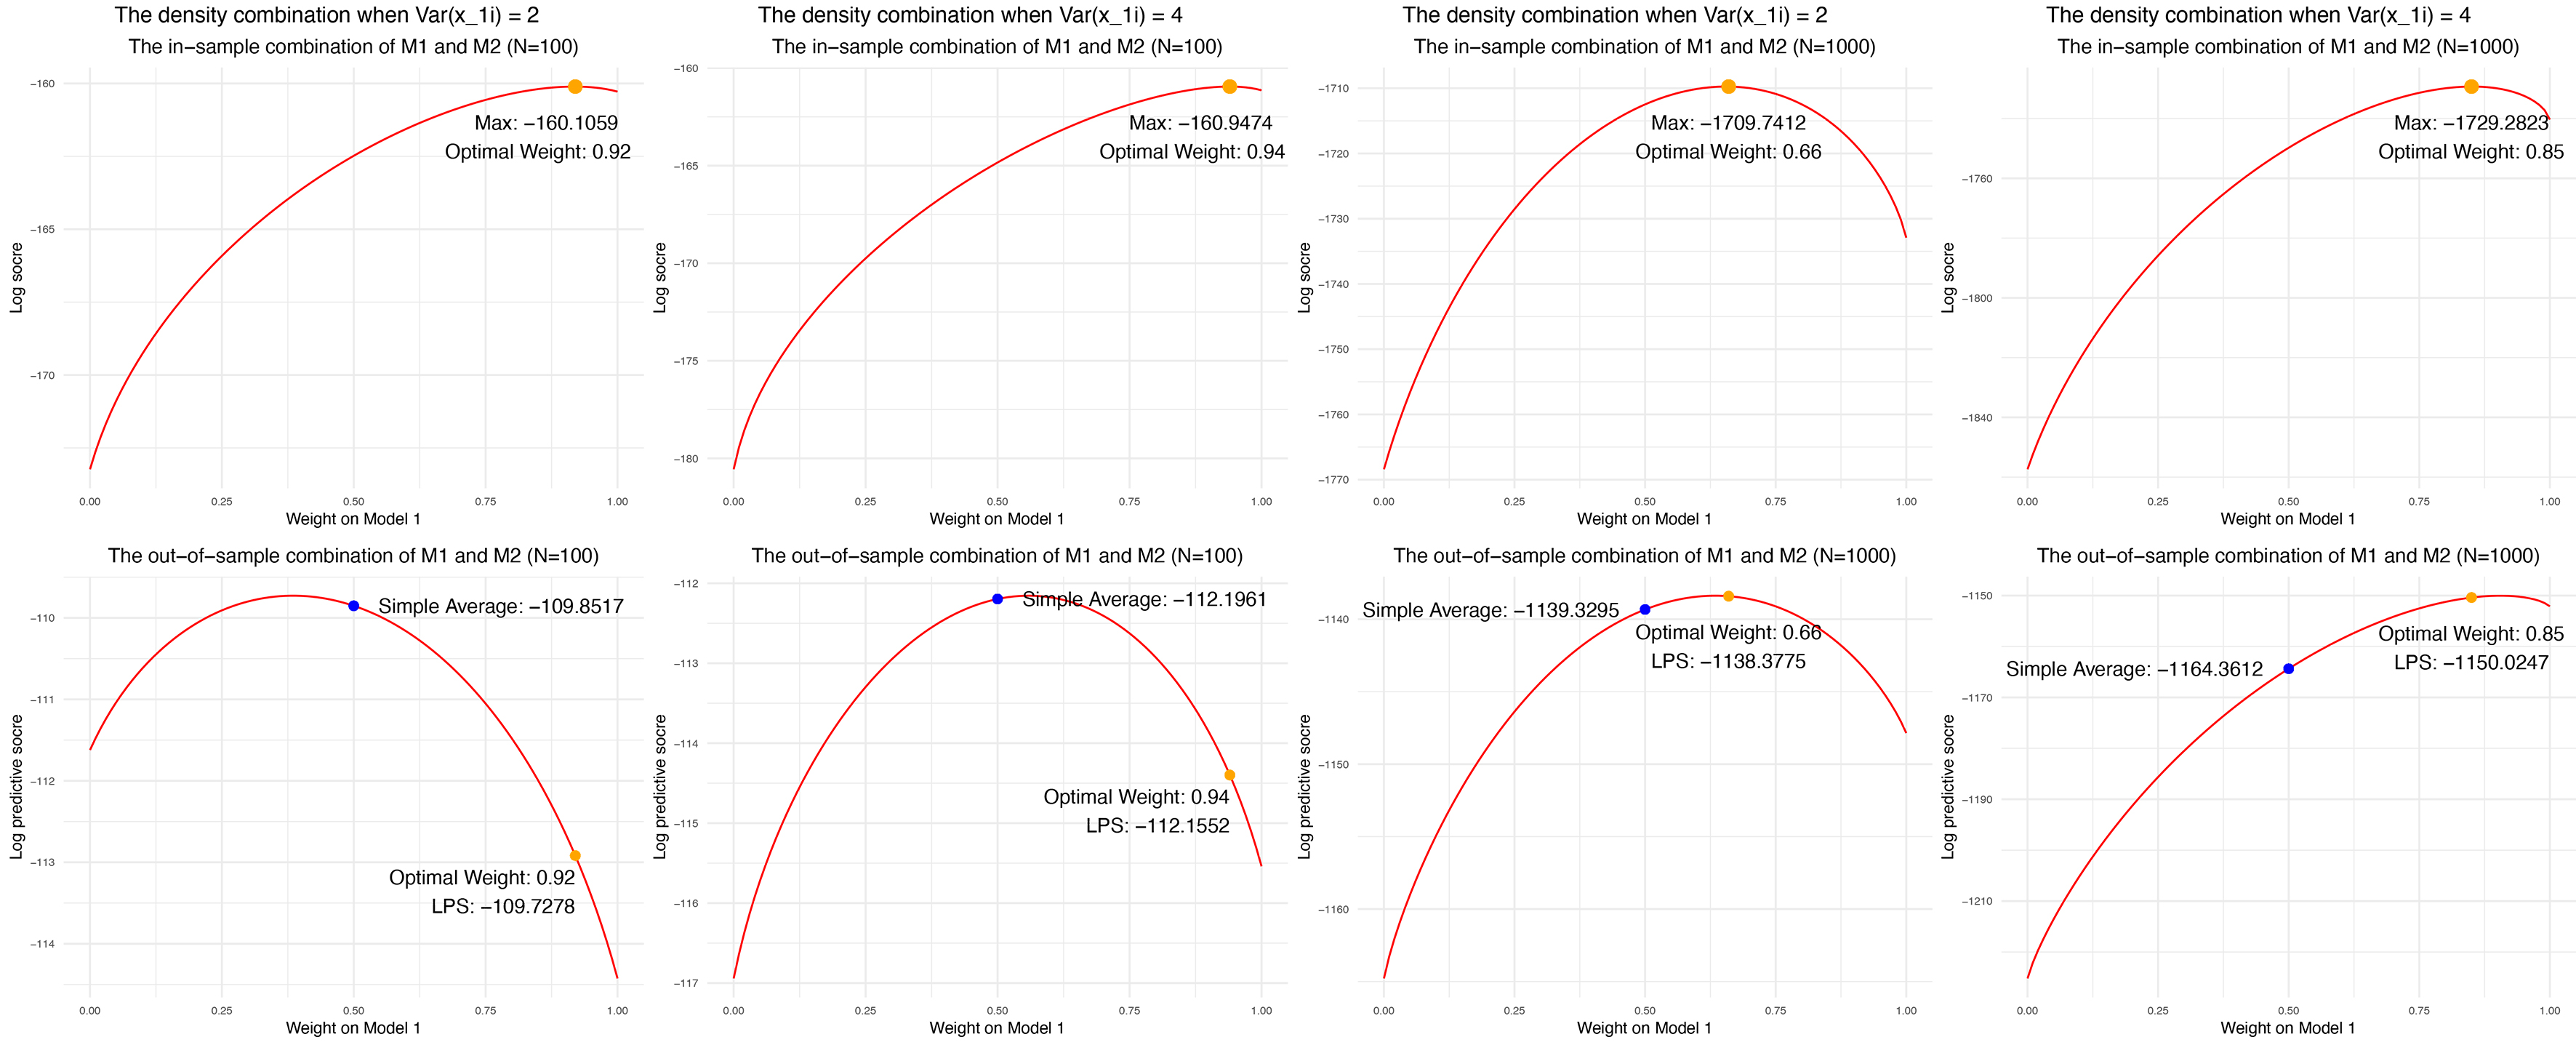
\includegraphics[scale=0.18, angle=90]{figures/var11.jpg}
\caption{The first and third columns $Var(x_{1i}) = 2$ and $Var(x_{2i}) = 1$. The second and fourth columns $Var(x_{1i}) = 4$ and $Var(x_{2i}) = 1$. The sample size is indicated in the subtitle. Other variables remain unchanged as in the initial set-up.}
\label{fig:variance}
\end{figure}

\printbibliography[title={Reference}]




\end{document}
